%%%%%%%%%%%%%%%%%%%%%%%%%%%%%%%%%%%%%%%%%%%%%%%%%%%%%%%%%%%%%%%%%%%%%%%%%%%%%%%%
% AMS Beamer series / Bologna FC / Template
% Andrea Omicini
% Alma Mater Studiorum - Università di Bologna
% mailto:andrea.omicini@unibo.it
%%%%%%%%%%%%%%%%%%%%%%%%%%%%%%%%%%%%%%%%%%%%%%%%%%%%%%%%%%%%%%%%%%%%%%%%%%%%%%%%
%\documentclass[handout]{beamer}\mode<handout>{\usetheme{default}}
%
\documentclass[presentation, 9pt]{beamer}\mode<presentation>{\usetheme{AMSBolognaFC}}
%\documentclass[handout]{beamer}\mode<handout>{\usetheme{AMSBolognaFC}}
%%%%%%%%%%%%%%%%%%%%%%%%%%%%%%%%%%%%%%%%%%%%%%%%%%%%%%%%%%%%%%%%%%%%%%%%%%%%%%%%
\usepackage[T1]{fontenc}
\usepackage{wasysym}
\usepackage{amsmath,blkarray}
\usepackage{soul}
\usepackage[minted,most]{tcolorbox}
\usepackage{centernot}
\usepackage{fontawesome}
\usepackage{fancyvrb}
\usepackage{minted}
\usepackage{hyperref}
\usepackage{multicol}
\setminted[scala]{fontsize=\small,frame=lines,baselinestretch=1,obeytabs=true, tabsize=2}
\setminted[yaml]{fontsize=\large,frame=lines,linenos,baselinestretch=1,obeytabs=true, tabsize=2}
\usepackage[ddmmyyyy]{datetime}
\setminted{fontsize=\footnotesize}
\renewcommand{\dateseparator}{}
%\renewcommand{\thefootnote}{\fnsymbol{footnote}}
\newcommand{\version}{1}

\usepackage[
	%backend=biber,
	backend=bibtex,
%	citestyle=authoryear-icomp,
%	maxcitenames=1,
	bibstyle=numeric,
	style=ieee]{biblatex}

	\makeatletter

%\addbibresource{biblio.bib}

\bibliography{biblio}


\newcommand\extrafootertext[1]{%
    \bgroup
    \renewcommand\thefootnote{\fnsymbol{footnote}}%
    \renewcommand\thempfootnote{\fnsymbol{mpfootnote}}%
    \footnotetext[0]{#1}%
    \egroup
}

\newcommand{\citeinslide}[1]{\cite{#1}\extrafootertext{\scriptsize\cite{#1} \fullcite{#1}}}


%%%%%%%%%%%%%%%%%%%%%%%%%%%%%%%%%%%%%%%%%%%%%%%%%%%%%%%%%%%%%%%%%%%%%%%%%%%%%%%%
\title[Programming with ScaFi!]
{Programming (and Learning) Self-Adaptive \& Self-Organising Behaviour with ScaFi}
\subtitle{for Swarms, Edge-Cloud Ecosystems, and More}
%
%
\author[\sspeaker{Casedei}]
{\speaker{Roberto Casadei} \href{mailto:roby.casadei@unibo.it}{roby.casadei@unibo.it} \\
\speaker{Gianluca Aguzzi} \href{mailto:gianluca.aguzzi@unibo.it}{gianluca.aguzzi@unibo.it} \\
\speaker{Danilo Pianini} \href{mailto:danilo.pianini@unibo.it}{danilo.pianini@unibo.it} \\
\speaker{Mirko Viroli} \href{mailto:mirko.viroli@unibo.it}{mirko.viroli@unibo.it}}
%
\institute[DISI, Univ.\ Bologna]
{%Dipartimento di Informatica -- Scienza e Ingegneria (DISI)\\
\textsc{Alma Mater Studiorum} -- Universit{\`a} di Bologna \\[0.1cm]
\textbf{Talk @} \bold{International Conference on Autonomic Computing and Self-Organizing Systems (ACSOS)}\\[0.15cm]

\includegraphics[width=0.15\textwidth]{img/qr-code-scafi.png}

\includegraphics[width=0.15\textwidth]{img/qr-code.png}
}
%
\renewcommand{\dateseparator}{/}
\date[\today]{\today}
%
\AtBeginSubsection[]
{
  \begin{frame}
  \frametitle{Contents}
  \tableofcontents[currentsubsection, 
	sectionstyle=show/shaded, 
	subsectionstyle=show/shaded]
  \end{frame}
}
\AtBeginSection[]
{
  \begin{frame}
  \frametitle{Contents}
  \tableofcontents[currentsubsection, 
	sectionstyle=show/shaded, 
	subsectionstyle=show/shaded]
  \end{frame}
}
%%%%%%%%%%%%%%%%%%%%%%%%%%%%%%%%%%%%%%%%%%%%%%%%%%%%%%%%%%%%%%%%%%%%%%%%%%%%%%%%



\lstdefinelanguage{scala}{
  keywords={abstract,case,catch,class,def,%
    do,else,extends,false,final,finally,%
    for,if,implicit,import,match,mixin,%
    new,null,object,override,package,%
    private,protected,requires,return,sealed,%
    super,this,throw,trait,true,try,lazy,%
    type,val,var,while,with,yield,forSome},
  otherkeywords={=>,<-,<\%,<:,>:,\#},
  sensitive=true,
  morecomment=[l]{//},
  morecomment=[n]{/*}{*/},
  morestring=[b]",
  morestring=[b]',
  morestring=[b]""",
  basicstyle=\lst@ifdisplaystyle\footnotesize\fi\ttfamily,
  emphstyle=\bfseries
}
\definecolor{ddarkgreen}{rgb}{0,0.5,0}
\lstdefinelanguage{scafi}{frame=single,basewidth=0.5em,language={scala},
keywordstyle=\color{blue}\textbf, commentstyle=\color{ddarkgreen},
keywordstyle=[2]\color{red}\textbf, keywords=[2]{rep,nbr,foldhood,foldhoodPlus,aggregate,branch,spawn},
keywordstyle=[3]\color{gray}, keywords=[3]{Me,AroundMe,Everywhere,Forever}, %,@@,@@@
keywordstyle=[4]\color{red}\textbf, keywords=[4]{in,out,rd},
keywordstyle=[5]\color{violet}, keywords=[5]{evolve,when,andNext,workflow,C,gossip},
keywordstyle=[6]\color{orange}, keywords=[6]{Available,Serving,Done,Waiting,Removing}}

\newcommand{\hsplit}[2]{
\begin{minipage}{0.48\textwidth}
#1
\end{minipage}
\hfill
\begin{minipage}{0.48\textwidth}
#2
\end{minipage}
}
\newcommand{\hsplits}[4]{
\begin{minipage}{#1\textwidth}
#3
\end{minipage}
\hfill
\begin{minipage}{#2\textwidth}
#4
\end{minipage}
}

\newcommand{\lbl}[1]{\textbf{\textcolor{gray!90!white}{#1}}}
\newcommand{\enf}[1]{{\textcolor{red}{#1}}}
\newcommand{\bo}[1]{\textbf{#1}}

\newcommand{\imgh}[2]{
\begin{figure}
\centering
\includegraphics[width=#1\textwidth]{img/#2}
\end{figure}
}
\newcommand{\imgv}[2]{
\begin{figure}
\centering
\includegraphics[height=#1\textheight]{img/#2}
\end{figure}
}

\newtcblisting{mycode}[3]{%
  boxsep=0pt,
  boxrule=0pt,
  arc=1mm, 
  left=1mm,
  %auto outer arc,
  size=fbox,%tight,
  %colframe=blue!40!black, colframe=black!30!white,
  %colbacktitle=blue!80!white,
  colback=blue!5,
  %toprule=0.1mm, bottomrule=0.1mm, rightrule=0.1mm, leftrule=1mm, 
  listing only,
  listing options={language=scala, alsoletter={-},
    backgroundcolor={},
  	columns=fullflexible,
  	lineskip={-1.5pt},
  	xleftmargin=0px,
  	belowskip={0px},
  	aboveskip={0px},
  	frame=none,
  	#2
  },
  title={#3},#1
}
\lstdefinestyle{s}{basicstyle=\ttfamily\footnotesize}
\lstdefinestyle{ss}{basicstyle=\ttfamily\scriptsize}
\lstdefinestyle{sss}{basicstyle=\ttfamily\tiny}
\lstdefinestyle{conf}{language={},morecomment=[l][\color{darkgreen}]{\#},
basicstyle=\ttfamily\scriptsize}



\begin{document}
%%%%%%%%%%%%%%%%%%%%%%%%%%%%%%%%%%%%%%%%%%%%%%%%%%%%%%%%%%%%%%%%%%%%%%%%%%%%%%%%
%!TeX root = presentation-2024-ap-toolchain.tex
%%% Syntax

\newcommand{\FieldS}[0]{\mathcal{F}}
\newcommand{\EventS}[0]{\mathcal{E}}
\newcommand{\eventS}[0]{E}
\newcommand{\timeS}[0]{t}
\newcommand{\posS}[0]{p}
\newcommand{\event}[3]{\langle #1,#2,#3\rangle}
\newcommand{\devF}[1]{\deviceId_{#1}}
\newcommand{\timeF}[1]{\timeS_{#1}}
\newcommand{\posF}[1]{\posS_{#1}}
\newcommand{\domS}[0]{D}
\newcommand{\DomS}[0]{\mathcal{D}}
\newcommand{\DomDevF}[2]{#1(#2)}
\newcommand{\DomTimeF}[2]{#1(#2)}
\newcommand{\DomMTimeF}[2]{#1^{-}(#2)}
\newcommand{\DomDomF}[2]{#1(#2)}
\newcommand{\DomDevTimeF}[3]{#1(#2,#3)}
\newcommand{\DomDevMTimeF}[3]{#1^{-}(#2,#3)}

\newcommand{\feS}[0]{\Phi}
\newcommand{\setVS}[0]{\textbf{V}}
\newcommand{\setTS}[0]{\textbf{T}}
\newcommand{\setCS}[0]{\textbf{C}}

\newcommand\pto{\mathrel{\ooalign{\hfil$\mapstochar$\hfil\cr$\to$\cr}}}

\newcommand{\neighbour}[2]{\textit{neigh}(#1,#2)}

\newcommand{\denot}[1]{\mathcal{E}\llbracket{#1}\rrbracket}
\newcommand{\denotapp}[2]{\denot{#1}_{#2}}
\newcommand{\denotappsub}[3]{\denot{#1}_{#2}^{#3}}
\newcommand{\denotfun}[3]{\mathcal{L}\llbracket{#1}\rrbracket_{#2}^{#3}}
\newcommand{\denottype}[1]{\mathcal{T}\llbracket{#1}\rrbracket}
\newcommand{\denotexp}[3]{\mathcal{E}\llbracket{#1}\rrbracket_{#2}^{#3}}
\newcommand{\denotf}[2]{\lambda #1.#2}

\newcommand{\dvalue}[0]{V}

\newcommand{\myeval}[4]{\epsilon(#1,#2,#3,#4)}

\newcommand{\fiecomp}[2]{#1[#2]}


\newcommand{\BNFcce}{{\bf ::=}}
\newcommand{\BNFmid}{\;\bigr\rvert\;}

\newcommand{\PROGRAM}{\texttt{P}}
\newcommand{\FUNCTION}{\texttt{F}}
\newcommand{\e}{\texttt{e}}
\newcommand{\fname}{\texttt{f}}
\newcommand{\xname}{\texttt{x}}
\newcommand{\yname}{\texttt{y}}
\newcommand{\oname}{\texttt{o}}
\newcommand{\pe}{\texttt{p}} % pure expression
\newcommand{\we}{\texttt{w}} % variable or (local) value




\newcommand{\asuper}{\texttt{s}}
\newcommand{\avalue}{\texttt{v}}
\newcommand{\bvalue}{\textit{b}}
\newcommand{\obvalue}{\option{\bvalue}}
\newcommand{\lvalue}{\texttt{l}}
\newcommand{\olvalue}{\option{\lvalue}}
\newcommand{\nvalue}{\texttt{n}}
\newcommand{\tvalue}{\texttt{t}}
\newcommand{\hvalue}{\texttt{h}}
\newcommand{\fvalue}{\phi}
\newcommand{\nolabel}{\_}
\newcommand{\fdom}[1]{\textit{dom}(#1)}
\newcommand{\oexec}{\epsilon}

\newcommand{\brvalue}{\textit{b}}
\newcommand{\obrvalue}{\option{\brvalue}}
\newcommand{\lrvalue}{\textit{l}}
\newcommand{\olrvalue}{\option{\lrvalue}}

\newcommand{\tvalueExt}[1]{(\lvalue_1,\ldots,\lvalue_{#1})}
\newcommand{\fvalueExt}[2]{\{#1\mapsto #2\}}
\newcommand{\fvalueOne}[2]{\{#1\mapsto #2\}}
\newcommand{\fvalueWrap}[1]{\{#1\}}
\newcommand{\fvaluewrapped}[2]{#1\mapsto #2}
\newcommand{\fvalues}[2]{#1\mapsto #2}
%\newcommand{\memslot}[2]{\{#1:=#2\}}
\newcommand{\memslot}[2]{#1:=#2}
\newcommand{\treeslot}[2]{#1\mapsto #2}
\newcommand{\emptyL}{\bullet}

\newcommand{\avalueSet}{\mathcal{V}}
\newcommand{\lvalueSet}{\mathcal{L}}
\newcommand{\nvalueSet}{\mathcal{N}}
\newcommand{\tvalueSet}{\mathcal{T}}
\newcommand{\hvalueSet}{\mathcal{H}}
\newcommand{\fvalueSet}{\Phi}
% Keywords
\newcommand{\defK}{\texttt{def}}
\newcommand{\nbrK}{\texttt{nbr}}
\newcommand{\repK}{\texttt{rep}}
\newcommand{\ifK}{\texttt{if}}

\newcommand{\tname}{\texttt{t}}

\newcommand{\ltrue}{\textit{t}}
\newcommand{\lfalse}{\textit{f}}


%%% Runtime Syntax

\newcommand{\wildcard}{{\cdots}} %%% non intresting syntact element
%\newcommand{\option}[1]{{{#1}_\mathit{opt}}} %%% optional syntact element
\newcommand{\option}[1]{\mathring{#1}} %%% optional
\newcommand{\evaluatedPlace}{{\place_\mathit{top}}} %%% optional syntact element
%%%\newcommand{\re}{\textit{r}} %%% runtime expression
\newcommand{\re}{\textit{a}} %%% runtime expression
\newcommand{\rv}{\textit{v}} %%% runtime value
\newcommand{\lre}{\textit{e}} %%% labeled runtime expression
\newcommand{\olre}{\option{\lre}} %%% optional labeled runtime expression
%%%\newcommand{\orv}{\textit{w}}  %%% optional runtime value
\newcommand{\orv}{\option{\rv}}  %%% optional runtime value
\newcommand{\ob}{\textit{b}}  %%% optional body
\newcommand{\Env}{\Gamma}
\newcommand{\emptyEnv}{\bullet}
\newcommand{\Trees}{\Theta}
\newcommand{\emptyTrees}{\bullet}
\newcommand{\labelled}[2]{#1\!\!\cdot\!\!{#2}}
\newcommand{\labelledsmall}[2]{#1\cdot{#2}}
\newcommand{\labelledC}[2]{#1^{#2}}
\newcommand{\labelledCsmall}[2]{#1^{#2}}

\newcommand{\he}{h} %%%  local value or runtime expression
\newcommand{\ohe}{\option{\he}} %%% optional local value or runtime expression
\newcommand{\ue}{\textit{u}} %%% unevaluated runtime expression
\newcommand{\uhe}{\option{\ue}} %%% optional unevaluated runtime expression

\newcommand{\unfoldK}{\texttt{unfold}}

\newcommand{\newopsem}[5]{#1;#2;#3\vdash #4\rightarrow #5}
\newcommand{\opsem}[4]{#1;#2\vdash #3\rightarrow #4}
\newcommand{\opsemmany}[4]{#1;#2\vdash #3\rightarrow^* #4}
\newcommand{\opsemNF}[3]{#1;#2\vdash #3\not\rightarrow}

\newcommand{\self}{\texttt{self}}

%%% Alignment contexts

\newcommand{\actx}{\mathbb{A}}
\newcommand{\matches}{::}

%%% Contexts

\newcommand{\ctxapp}[2]{#1[#2]}
\newcommand{\ctxappfull}[3]{\ctxapp{#1}{#2}\langle #3\rangle}
\newcommand{\ctx}{\mathbb{C}}
\newcommand{\ctxr}{\mathbb{R}}
\newcommand{\ctxf}{\mathbb{N}}
\newcommand{\ctxc}{\mathbb{C}}
\newcommand{\ctxrt}{\mathbb{RT}}
\newcommand{\ctxt}{\mathbb{T}}
\newcommand{\ctxre}{\mathbb{RE}}
\newcommand{\ctxe}{\mathbb{E}}
\newcommand{\hole}{[]}
\newcommand{\place}{\langle\rangle}
\newcommand{\placefilled}[1]{\langle #1\rangle}
\newcommand{\inversectx}[2]{\spi{#1}(#2)}
\newcommand{\spi}[1]{\pi_{#1}}
\newcommand{\erase}[1]{|#1|}

\newcommand{\transition}[3]{
  \begin{array}{l@{\;}c}
    \stackrel{~}{{\tiny \textrm{[#1]}}} & #2 \\ \hline
    \multicolumn{2}{c}{#3}
  \end{array}
}
\newcommand{\transitiontwoprec}[4]{
  \begin{array}{l@{\qquad}c}
    & #2\\
    {\tiny \textrm{[#1]}} & #3 \\ \hline
    \multicolumn{2}{c}{#4}
  \end{array}
}
\newcommand{\nulltransition}[2]{
  \transition{#1}{}{#2}
}

\newcommand{\smallerskiptransition}{\\[-4pt]}
\newcommand{\smallskiptransition}{\\[0pt]}
\newcommand{\skipreduction}{\\}
\newcommand{\skiptransition}{\\[10pt]}
\newcommand{\bigskiptransition}{\\[15pt]}

\newcommand{\sta}{\textit{s}}
\newcommand{\stat}[4]{\langle#1,#2,#3,#4\rangle}
\newcommand{\topStat}[3]{\langle#1,#2,#3\rangle}
\newcommand{\tstat}[5]{#1\!::\!\langle #2,#3,#4,#5\rangle}
\newcommand{\msg}[2]{\{#1\rhd #2\}}
\newcommand{\fullmsg}[3]{#1:#2\rhd #3}
\newcommand{\sys}{\textit{N}}
\newcommand{\opar}{\;||\;}
\newcommand{\opard}{\oplus}
\newcommand{\lab}{\lambda}
\newcommand{\labtau}[1]{#1:\tau}
\newcommand{\labstart}[2]{#1\uparrow #2}
\newcommand{\labstop}[3]{#1\downarrow(#3) #2}
\newcommand{\upd}[2]{#1[#2]}
\newcommand{\replace}[2]{#2\rhd #1}
\newcommand{\proj}[2]{{#1}|_{#2}}
\newcommand{\topo}{\varSigma}
\newcommand{\envmap}[2]{\{#1\mapsto #2\}}

\newcommand{\fromMsg}[2]{\mathit{from}(#1,#2)}
\newcommand{\toMsg}[2]{\mathit{to}(#1,#2)}

\newcommand{\initNAME}{\textit{init}}
\newcommand{\init}[1]{\initNAME(#1)}
\newcommand{\ruleNameSize}[1]{{\scriptsize #1}}

\newcommand{\shadow}[1]{{\it \textcolor{gray}{#1}}} % inline comment

% Code highlighting
\newcommand{\il}[1]{{\it \textcolor{gray}{;; #1}}} % inline comment
\newcommand{\km}[1]{{\bf \textcolor{red}{#1}}} % key mechanism primitives
\newcommand{\fn}[1]{\textcolor{blue}{#1}} % function calls
\newcommand{\pr}[1]{\textcolor{magenta}{#1}} % primitives
\newcommand{\bk}[1]{{\bf\fn{#1}}} % primitives

%values

\newcommand{\somevalue}{\texttt{w}}
\newcommand{\anyvalue}{\texttt{v}}
\newcommand{\anyvaluealt}{\texttt{u}}
\newcommand{\anyvaluebis}{\texttt{w}}
\newcommand{\anyvalueInNC}[2]{\anyvalue_{#1 (\textrm{in }#2)}}
\newcommand{\nullvalue}{\texttt{null}}
\newcommand{\propervalue}{\texttt{w}}
\newcommand{\numvalue}{\texttt{n}}
\newcommand{\stringvalue}{\texttt{s}}
\newcommand{\boolvalue}{\texttt{b}}
\newcommand{\groundvalue}{\texttt{g}}
\newcommand{\pairvalue}[2]{\langle#1,#2\rangle}


%sensors
%\newcommand{\snsname}{\texttt{\#sns}}
%\newcommand{\snsname}{s}
\newcommand{\snsname}{\texttt{Sns}}

%operators and functions
\newcommand{\pname}{\texttt{p}}
\newcommand{\main}{\texttt{main}}

%constructs
\newcommand{\spreadK}{\texttt{spread}}
\newcommand{\spreadTwo}[2]{\spreadK(#1:#2(*))}
%\newcommand{\spreadThree}[3]{\spreadK(#1\wedge#2(*,#3))}
\newcommand{\starK}{\texttt{@}}
\newcommand{\progK}[2]{#1(\starK,#2)}
\newcommand{\spreadThree}[3]{\{#1:\progK{#2}{#3}\}}

\newcommand{\saaK}{\texttt{grd}}
\newcommand{\saaTwo}[2]{\saaK(#1,#2)}
\newcommand{\saaThree}[3]{\saaK(#1,#2,#3)}

%typing functions and predicates
\newcommand{\lengthOf}[1]{\textit{length}(#1)}
\newcommand{\sizeOf}[1]{\textit{size}(#1)}
\newcommand{\signature}{\textit{signature}}
\newcommand{\signatureOf}[1]{\signature(#1)}
\newcommand{\bsWFTE}[4]{\textit{WFTE}(#1,#2,#3,#4)}

%types
\newcommand{\anytype}{\texttt{T}}
\newcommand{\nulltype}{\texttt{any}}
\newcommand{\numtype}{\texttt{mumber}}
\newcommand{\booltype}{\texttt{boolean}}
\newcommand{\stringtype}{\texttt{string}}
\newcommand{\pairtype}[2]{(#1\star#2)}

%type semantics
\newcommand{\lsempar}{[\![}
\newcommand{\rsempar}{]\!]}
\newcommand{\semOf}[1]{\lsempar{#1}\rsempar}
\newcommand{\lowerBound}{\textstyle{\bigwedge}}
\newcommand{\lowerBoundWith}[1]{\lowerBound_{#1}}

\newcommand{\suitableProse}{locally noetherian}
\newcommand{\suitableTypeText}{lnoe}
%\newcommand{\SuitableTypeText}{Noe}
\newcommand{\suitableType}{\suitableTypeText}
\newcommand{\suitableTypeOf}[1]{\suitableType(#1)}
\newcommand{\suitableOpText}{suitable}
\newcommand{\SuitableOpText}{stabilising}
\newcommand{\suitableOp}{\SuitableOpText}
\newcommand{\suitableOpOf}[1]{\suitableOp(#1)}


\newcommand{\wfLt}{<}
\newcommand{\wfLtOf}[1]{\wfLt_{#1}}
\newcommand{\wfLe}{\le}
\newcommand{\wfLeOf}[1]{\wfLe_{#1}}

\newcommand{\wfGt}{>}
\newcommand{\wfGtOf}[1]{\wfGt_{#1}}
\newcommand{\wfGe}{\ge}
\newcommand{\wfGeOf}[1]{\wfGe_{#1}}

\newcommand{\neginf}{\texttt{bottom}}
\newcommand{\neginfOf}[1]{\neginf(#1)}
\newcommand{\posinf}{\texttt{top}}
\newcommand{\posinfOf}[1]{\posinf(#1)}
\newcommand{\initial}{\texttt{default}}
\newcommand{\initialOf}[1]{\initial(#1)}
\newcommand{\topvalue}{\top}
\newcommand{\topvalueOf}[1]{\topvalue_{#1}}
\newcommand{\TypeDouble}{\texttt{Double}}
\newcommand{\topvalueOfDouble}[1]{\topvalue_{#1}}

%semantic functions and predicates
\newcommand{\minimize}{\textit{min}}
\newcommand{\minimizeOf}[1]{\minimize_{#1}}
\newcommand{\dom}{\textit{dom}}
\newcommand{\domOf}[1]{\dom(#1)}
\newcommand{\noetherian}{\textit{noetherian}}
\newcommand{\noetherianOf}[1]{\noetherianOf(#1)}
\newcommand{\noetherianOrd}{<}
\newcommand{\noetherianOrdOf}[1]{\noetherianOrd_{#1}}
\newcommand{\progressive}{\textit{Progressive}}
\newcommand{\progressiveOf}[1]{\progressive(#1)}
\newcommand{\sense}[2]{#1(#2)}

%small-step network operational semantic
\newcommand{\netframe}{\Envi}
\newcommand{\mknetframe}[3]{(#1,#2,#3)}
\newcommand{\netframeName}{\textit{environment}}
\newcommand{\netframeOf}[1]{\netframeName(#1)}
\newcommand{\stablencOf}[1]{R_{#1}}
%\newcommand{\stablencOf}[1]{\textit{snc}(#1)}

\newcommand{\deviceIdSet}{\textbf{D}}
\newcommand{\nodeSubSet}{\textbf{C}}
\newcommand{\stableNodeSet}{\textbf{S}}
\newcommand{\network}{\Cfg}
\newcommand{\netRestrict}[2]{#1|_{#2}}
\newcommand{\initialNetwork}{\mathcal{I}}
\newcommand{\stableNetwork}{R}
\newcommand{\mkgraph}[2]{(#1,#2)}
\newcommand{\mknetwork}[4]{(#1,#2,#4,#3)}
\newcommand{\nodeSet}{\textbf{N}}
\newcommand{\edgeSet}{\textbf{E}}
\newcommand{\stateMap}{\Delta}
\newcommand{\statePair}[2]{(#1,#2)}
\newcommand{\stateMapPair}[2]{(#1,#2)}
\newcommand{\snsFunMap}{\Sigma}
\newcommand{\topSnsFun}{\tau}
\newcommand{\InitialSnsFun}[1]{\textit{Initial}(#1)}
%\newcommand{\topSnsFun}{\snsFun_{\posinf}}
\newcommand{\snsFun}{\sigma}
\newcommand{\snsFunFor}[1]{\snsFun_{#1}}
\newcommand{\snsFunOf}[1]{\snsFunMap(#1)}
\newcommand{\snsFunMapPair}[2]{(#1,#2)}
\newcommand{\snsFunPair}[2]{(#1,#2)}
\newcommand{\mkedge}[2]{(#1,#2)}
\newcommand{\neigh}{\textit{neighbours}}
\newcommand{\neighOfIn}[2]{\neigh(#1,#2)}
\newcommand{\neighTE}{\textit{nvte}}
\newcommand{\neighTEOfIn}[3]{\neighTE(#1,#2,#3)}
\newcommand{\Disconnected}{\textit{Disconnected}}
\newcommand{\DisconnectedOfIn}[2]{\Disconnected(#1,#2)}
\newcommand{\codom}{\textit{codom}}
\newcommand{\codomOf}[1]{\codom(#1)}
\newcommand{\frontier}{\textit{frontier}}
\newcommand{\frontierOfIn}[2]{\frontier_{#1}(#2)}
\newcommand{\netopsemarrow}{\longrightarrow}
\newcommand{\netopsemarrowWith}[1]{\longrightarrow_{#1}}
\newcommand{\netopsemarrowStar}{\netopsemarrow^{\star}}
\newcommand{\netopsemarrowPlus}{\netopsemarrow^{+}}
\newcommand{\netopsem}[2]{#1\netopsemarrow#2}
\newcommand{\netopsemStar}[2]{#1\netopsemarrowStar#2}
\newcommand{\netopsemPlus}[2]{#1\netopsemarrowPlus#2}
\newcommand{\netopsemWith}[3]{#2\netopsemarrowWith{#1}#3}
\newcommand{\netopsemWithStar}[3]{#2\netopsemarrowWith{#1}#3}
\newcommand{\netopsemWithPlus}[3]{#2\netopsemarrowWith{#1}#3}
\newcommand{\netopsemRule}[3]{\surfaceTyping{#1}{#2}{#3}}
\newcommand{\nullnetopsemRule}[2]{\nullsurfaceTyping{#1}{#2}}
%\newcommand{\evaluationTrace}{\theta}
\newcommand{\initialvtree}{\theta_{\main}}
\newcommand{\vtree}{\theta}
\newcommand{\vtreealt}{\eta}
\newcommand{\vtreeInNC}[2]{\theta_{#1( \textrm{in }#2)}}
\newcommand{\initialTraceFor}[1]{\evaluationTrace_{#1}}
\newcommand{\traceFor}[4]{\evaluationTrace_{(#1,#2,#3,#4)}}
\newcommand{\donotcare}{\_}
\newcommand{\ruleName}{\textbf{r}}
\newcommand{\ruleNameSet}{\textbf{R}}
\newcommand{\senstate}{\sigma}
\newcommand{\genmap}[2]{#1\rhd#2}


\newcommand{\act}{\textit{act}}
\newcommand{\envact}{\textit{env}}
\newcommand{\netArr}{\rightarrow}
\newcommand{\netRed}[2]{#1\netArr#2}
\newcommand{\netArrAct}{\stackrel{\act}{\netArr}}
\newcommand{\netRedAct}[2]{#1\netArrAct#2}
\newcommand{\netArrWithAct}[1]{\stackrel{#1}{\netArr}}
\newcommand{\trueUpd}{\textsf{true}}
\newcommand{\falseUpd}{\textsf{false}}
\newcommand{\isUpd}{\textsf{b}}

\newcommand{\netArrStar}{\Longrightarrow}
%\newcommand{\netArrStar}{\longrightarrow^{\star}}
\newcommand{\netArrActStar}{\stackrel{\overline{\act}}{\netArrStar}}
%\newcommand{\netArrActStar}{\xrightarrow{\overline{\act}}^{\star}}
\newcommand{\netArrWithActStar}[1]{\stackrel{#1}{\netArrStar}}
%\newcommand{\netArrWithActStar}[1]{\xrightarrow{#1}^{\star}}

\newcommand{\netRedStar}[2]{#1\netArrStar#2}
\newcommand{\netRedWithActStar}[3]{#2\netArrWithActStar{#1}#3}

\newcommand{\pres}{\not\epsilon}
\newcommand{\netArrPres}{\netArr_{\pres}}
\newcommand{\netArrPresStar}{\netArrStar}
\newcommand{\netArrActPres}{\netArrAct}
\newcommand{\netArrActPresStar}{\netArrActStar}
\newcommand{\netArrWithActPresStar}[1]{\stackrel{#1}{\netArrStar}}

\newcommand{\firing}{\textit{firing}}
\newcommand{\fair}{\textit{fair}}
\newcommand{\Fair}{\textit{Fair}}

\newcommand{\fairsym}{\star}
\newcommand{\netArrFairStar}{\netArrStar_{\fairsym}}
\newcommand{\netArrActFairStar}{\netArrActStar_{\fairsym}}
\newcommand{\netArrFairStarN}[1]{\netArrStar_{#1}}
\newcommand{\netArrActFairStarN}[1]{\netArrActStar_{#1}}
\newcommand{\netRedFairStar}[2]{#1\netArrFairStar#2}
\newcommand{\netRedActFairStar}[2]{#1\netArrActFairStar#2}
\newcommand{\netRedActFairStarN}[3]{#2\netArrActFairStarN{#1}#3}


\newcommand{\actDevIn}{\textsf{di}}
%\newcommand{\actDevInOf}[1]{\actDevIn(#1)}
\newcommand{\actDevInOf}[1]{\envact}
\newcommand{\netArrDevInOf}[1]{\netArrWithAct{\actDevInOf{#1}}}
\newcommand{\netRedDevInOf}[3]{#2\netArrWithAct{\actDevInOf{#1}}#3}

\newcommand{\actDevOut}{\textsf{do}}
%\newcommand{\actDevOutOf}[1]{\actDevOut(#1)}
\newcommand{\actDevOutOf}[1]{\envact}
\newcommand{\netArrDevOutOf}[1]{\netArrWithAct{\actDevOutOf{#1}}}
\newcommand{\netRedDevOutOf}[3]{#2\netArrWithAct{\actDevOutOf{#1}}#3}

\newcommand{\actEdgeIn}{\textsf{ei}}
%\newcommand{\actEdgeInOf}[1]{\actEdgeIn(#1)}
\newcommand{\actEdgeInOf}[1]{\envact}
\newcommand{\netArrEdgeInOf}[1]{\netArrWithAct{\actEdgeInOf{#1}}}
\newcommand{\netRedEdgeInOf}[3]{#2\netArrWithAct{\actEdgeInOf{#1}}#3}

\newcommand{\actEdgeOut}{\textsf{eo}}
%\newcommand{\actEdgeOutOf}[1]{\actEdgeOut(#1)}
\newcommand{\actEdgeOutOf}[1]{\envact}
\newcommand{\netArrEdgeOutOf}[1]{\netArrWithAct{\actEdgeOutOf{#1}}}
\newcommand{\netRedEdgeOutOf}[3]{#2\netArrWithAct{\actEdgeOutOf{#1}}#3}

\newcommand{\actSnsUpd}{\textsf{su}}
%\newcommand{\actSnsUpdOf}[1]{\actSnsUpd(#1)}
\newcommand{\actSnsUpdOf}[1]{\envact}
\newcommand{\netArrSnsUpdOf}[1]{\netArrWithAct{\actSnsUpdOf{#1}}}
\newcommand{\netRedSnsUpdOf}[3]{#2\netArrWithAct{\actSnsUpdOf{#1}}#3}

\newcommand{\actDevUpd}{\textsf{df}}
%\newcommand{\actDevUpdOf}[1]{\actDevUpd(#1)}
\newcommand{\actDevUpdOf}[1]{#1}
\newcommand{\netArrDevUpdOf}[1]{\netArrWithAct{\actDevUpdOf{#1}}}
\newcommand{\netRedDevUpdOf}[3]{#2\netArrWithAct{\actDevUpdOf{#1}}#3}

%big-step device operational semantic
\newcommand{\resPair}[2]{#1,\,#2}
\newcommand{\emain}{\e_{\main}}
\newcommand{\opFun}{\epsilon}
%\newcommand{\opFunOf}[1]{\opFun_{#1}}
\newcommand{\opFunOf}[1]{\semOf{#1}}
\newcommand{\opApply}[2]{#1(#2)}
\newcommand{\neighSet}{\Theta}
\newcommand{\labe}{\texttt{l}}
\newcommand{\mklabe}[2]{#1[#2]}
\newcommand{\bsopsem}[4]{#1;#2\vdash #3\Downarrow #4}
\newcommand{\deviceId}{\delta}
\newcommand{\deviceIdalt}{\kappa}
\newcommand{\evaluationDerivation}{\mathcal{D}}
\newcommand{\evaluationDerivationFor}[4]{\evaluationDerivation_{(#1,#2,#3,#4)}}
\newcommand{\abstractJud}[3]{\treeslot{#1}{#2\downarrow#3}}
\newcommand{\premise}{\mathbf{\pi}}
\newcommand{\premiseNum}[1]{\premise_{#1}}
\newcommand{\premiseNumOf}[2]{\premiseNum{#1}(#2)}
\newcommand{\conclusion}{\mathbf{\rho}}
\newcommand{\conclusionOf}[1]{\conclusion(#1)}
\newcommand{\vroot}{\mathbf{\rho}}
\newcommand{\vrootOf}[1]{\vroot(#1)}
\newcommand{\substitution}[2]{#1:=#2}
\newcommand{\applySubstitution}[2]{#1[#2]}
\newcommand{\trace}{\textit{trace}}
\newcommand{\traceOf}[1]{\trace(#1)}

\frame{\titlepage}
%===============================================================================
\section{Introduction}
%%%%%%%%%%%%%%%%%%%%%%%%%%%%%%%%%%%%%%%%%%%%%%%%%%%%%%%%%%%%%%%%%%%%%%%%%%%
\subsection{Context -- Collective Adaptive Systems}
\begin{frame}{Context}
\begin{exampleblock}{Modern IT systems are more and more \bold{complex}}
	\begin{itemize}
		\item increasing availability of wearable/mobile/embedded/flying devices
		\item increasing availability of heterogeneous wireless networks
		\item increasing availability of computational resources (edge/fog/cloud computing)
		\item increasing production of data \bold{everywhere} and \bold{anytime}
	\end{itemize}
\end{exampleblock}
\begin{alertblock}{The challenge}
	Consider the worst-case possible scenario
	\begin{itemize}
		\item \bold{zillion} of devices \emph{unpredictably} locaed and moving in a space
		\item heterogeneous displacement, \bold{pervasive} sensing/actuation
		\item computational services are \bold{contextual} (proximity-based) and \emph{dynamic} 
	\end{itemize}
\end{alertblock}
\begin{center}
\Large{How can we \bold{program} such systems?}
\end{center}
\begin{center}
	\Large{What are the right \bold{abstractions}?}
	\end{center}
\end{frame}
\begin{frame}[plain,c]
	\begin{center}
	{\Huge \textbf{Collective Adaptive Systems} (CASs)}\\
	{\large Systems composed of \emph{possibly} \bold{large} set of component executing a \bold{collective} task strongly relying on component \bold{interactions} and showing \bold{inherent} \emph{adaptivity}.}\\[0.3cm]
	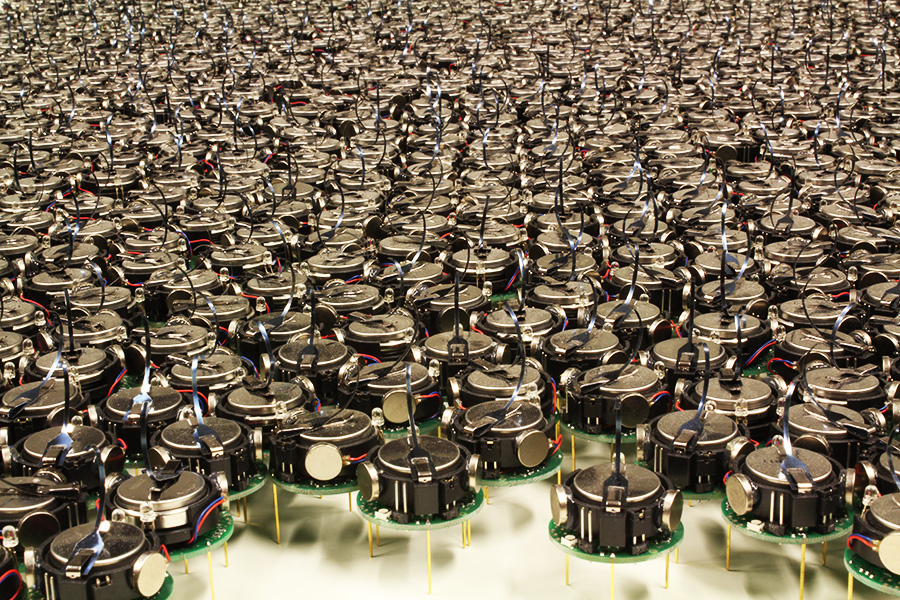
\includegraphics[width=0.28\textwidth]{img/swarms.jpg}
	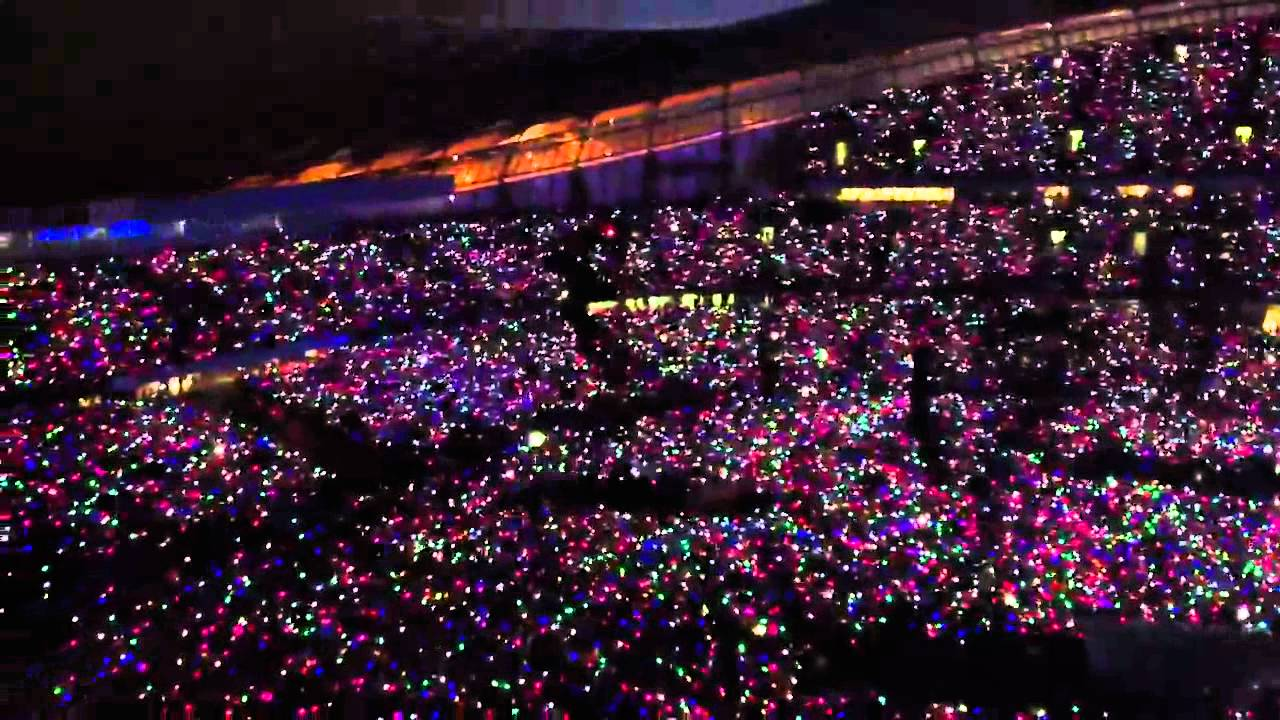
\includegraphics[width=0.333\textwidth]{img/coldplay.jpg}
	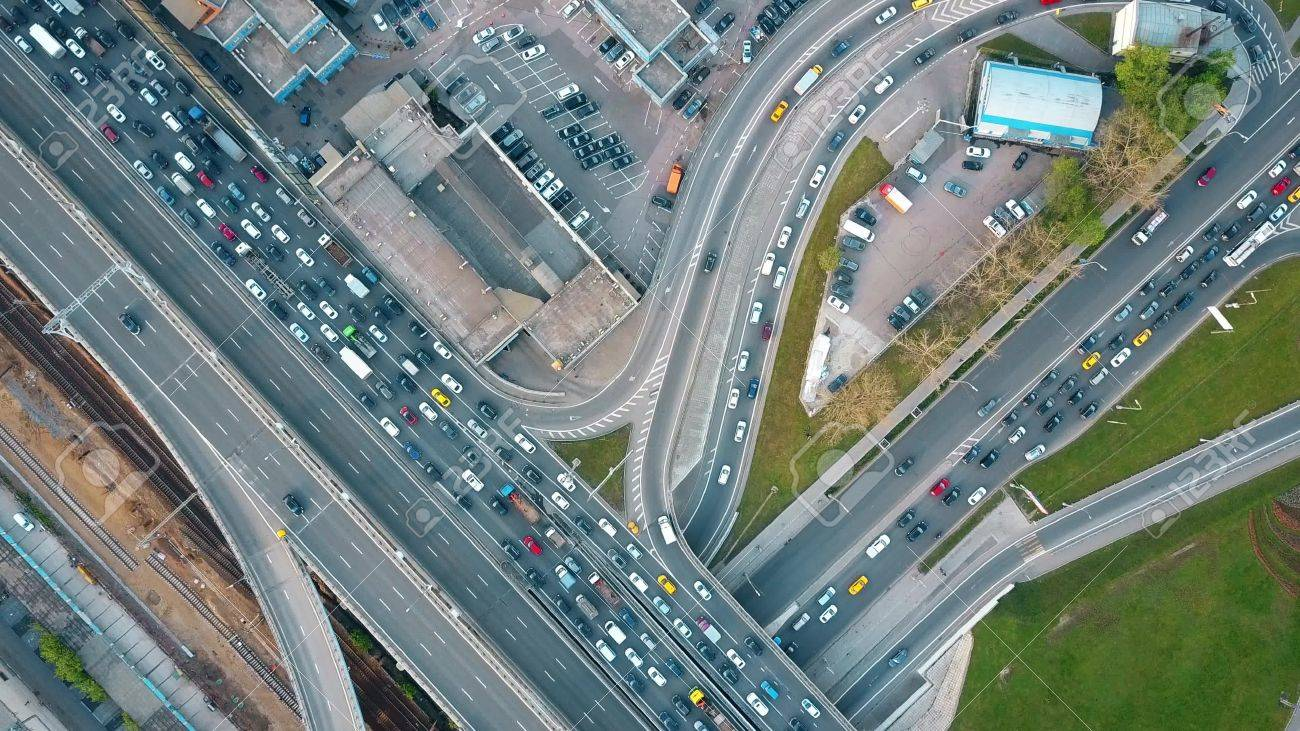
\includegraphics[width=0.333\textwidth]{img/traffic.jpg}	
	\end{center}
\end{frame}
\begin{frame}{Examples: controlling a fleet of drones}
\centering
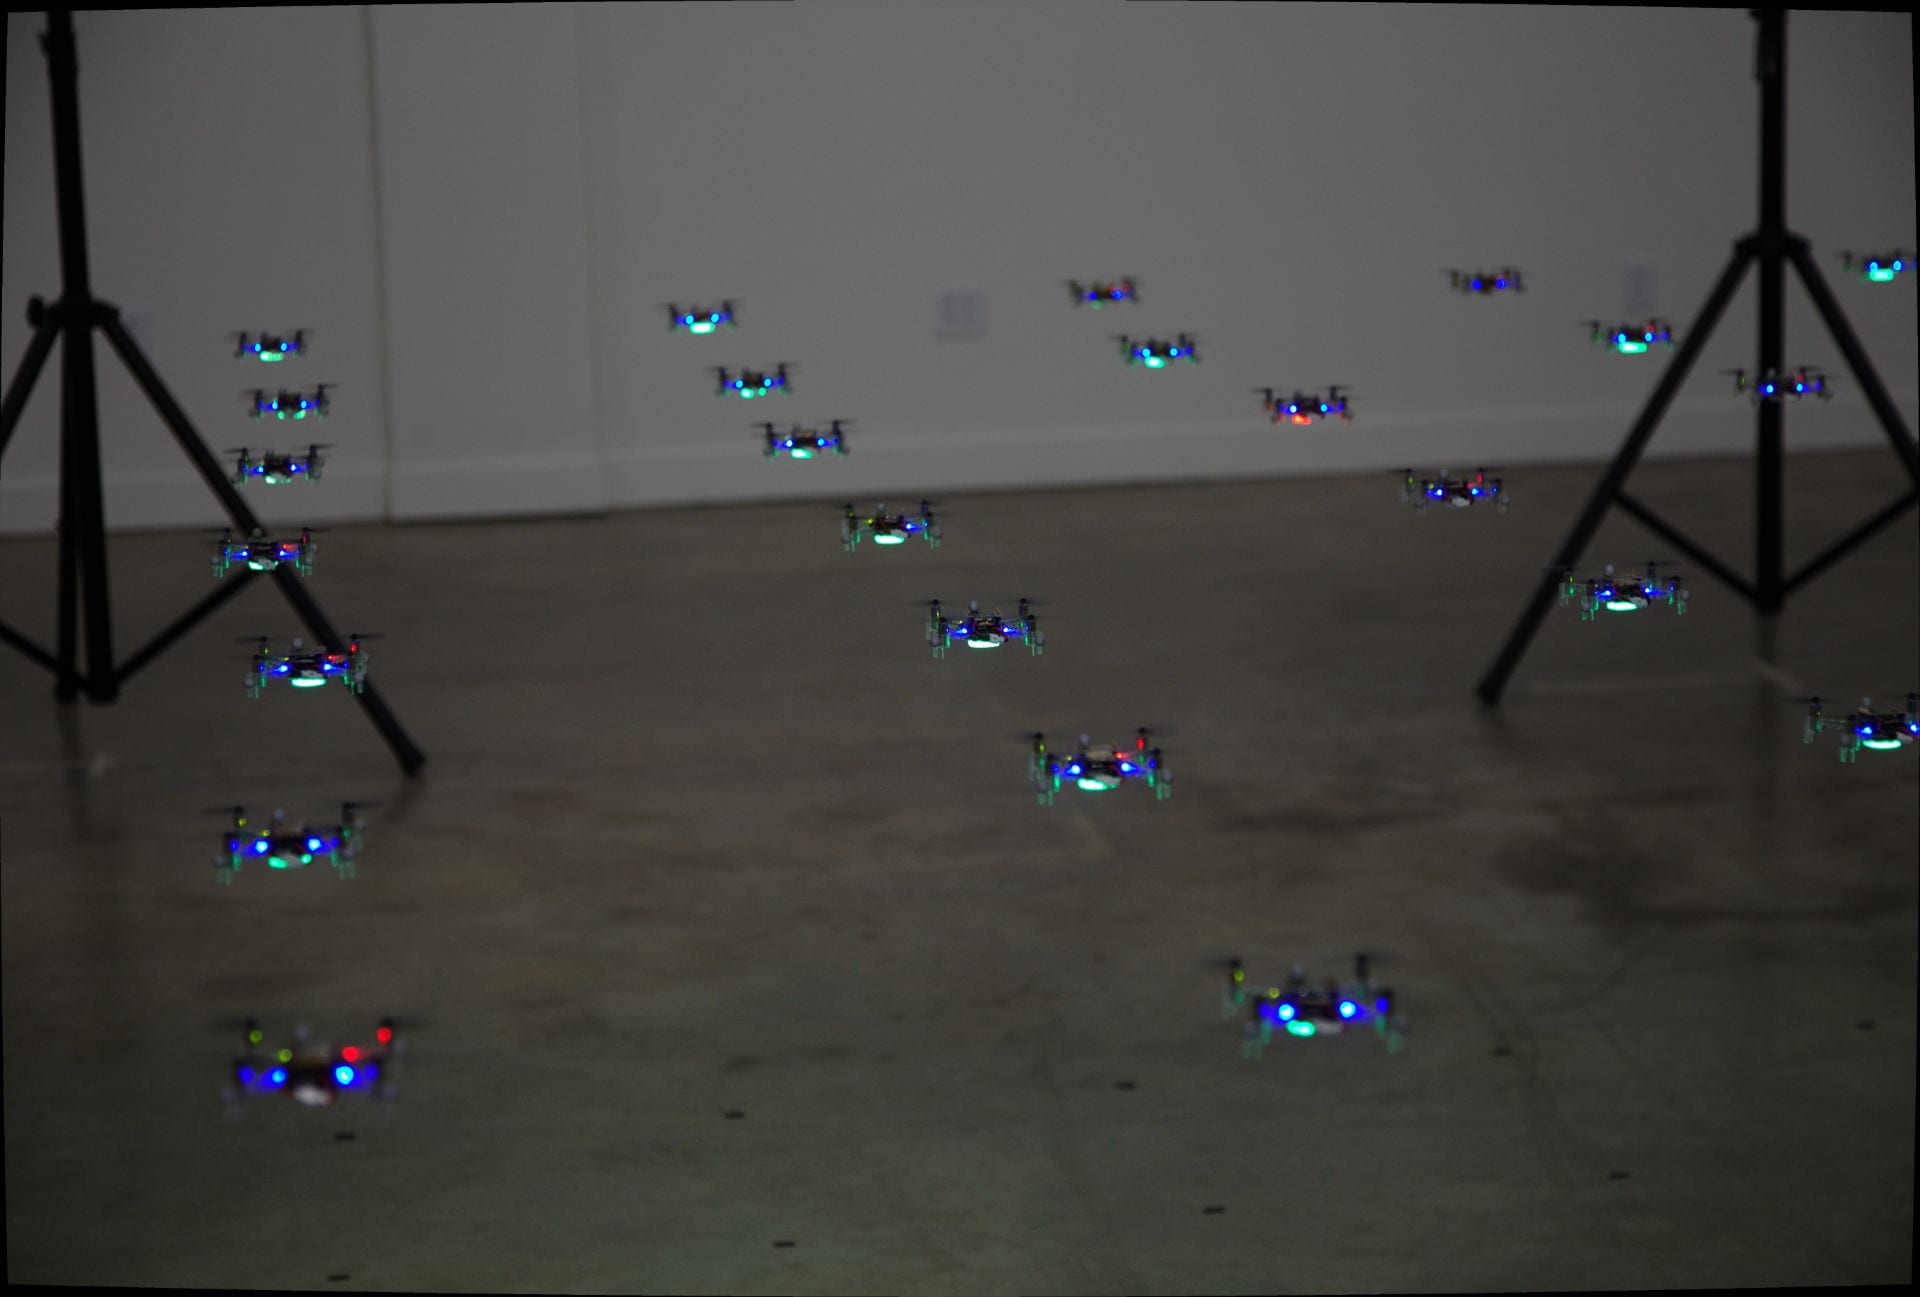
\includegraphics[width=0.7\textwidth]{img/crazyflies}
\begin{alertblock}{Issues}
\begin{itemize}
	\item Design techniques to \bold{reactively} propagate information across the fleet
	\item Create algorithms for \bold{higher-level} programming of the fleet
\end{itemize}
\end{alertblock}
\end{frame}
\begin{frame}{Examples: pedestrian steering in (smart)cities}
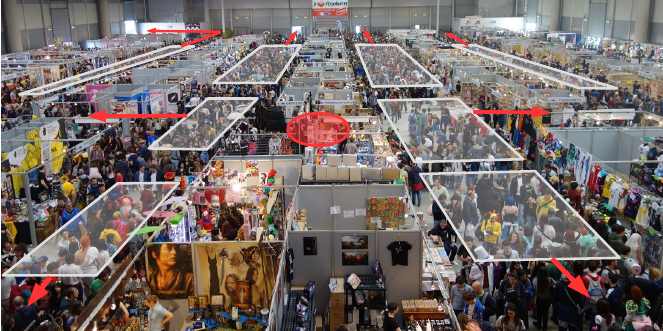
\includegraphics[width=0.9\textwidth]{img/pedastrian.png}
\begin{alertblock}{Issue}
	\begin{itemize}
		\item Design \bold{self-organisation} algorithms for people navigation
		\item More generally, design map-based large-scale applications
	\end{itemize}
\end{alertblock}
\end{frame}
\begin{frame}{Examples: fine control of crowds}
\centering
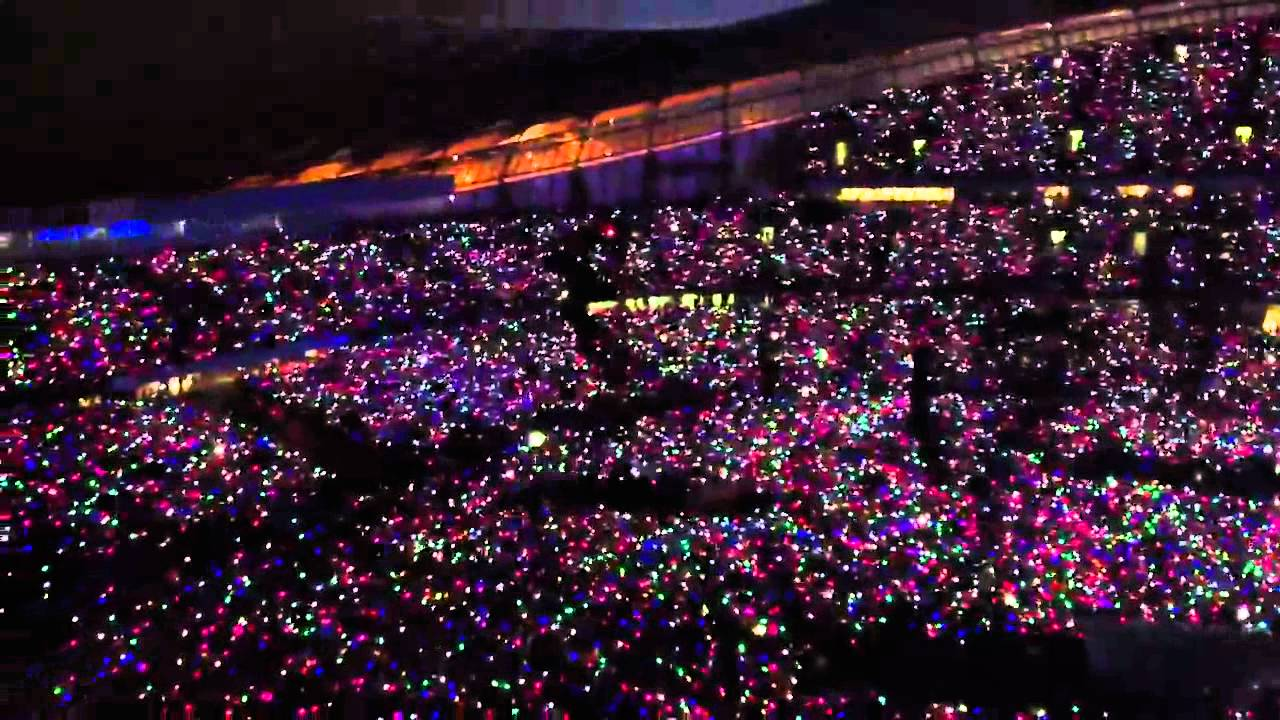
\includegraphics[width=0.9\textwidth]{img/coldplay}
\begin{alertblock}{Issues}
	\begin{itemize}
		\item Evaluating the influence of environment in crowd formation
		\item Evaluating the influence of ambient sensors, cameras and wearable
		devices
	\end{itemize}
\end{alertblock}
\end{frame}
\begin{frame}{Collective \underline{Adaptive} Systems}
\begin{alertblock}{\textbf{Adaptation}}
A system is \emph{adaptive} if it can \bold{change} its behaviour
depending on \bold{circumstances}, in order to better reach its \emph{goal}\\
\faArrowRight \, Adaptivess in \bold{intrisic} to open complex system (like CASs)
\end{alertblock}
\begin{exampleblock}{Kind of adaptiveness, self-* properties}
	\centering
	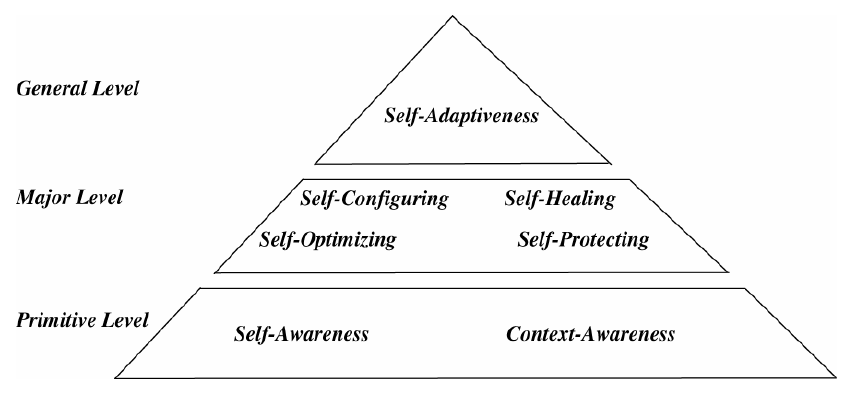
\includegraphics[width=0.8\textwidth]{img/self-*.png}
\end{exampleblock}
\end{frame}
\begin{frame}{Kind of adaptiveness}
\begin{exampleblock}{Self-adaptiveness: general level}
	\begin{itemize}
		\item \bold{self-adaptiveness} \faArrowRight \, the ultimate property we perceive from outside
		\item the terms ``self-*'' recalls a property achieved in \bold{autonomy}
		\item subcases: self-managing, -governing, -maintenance, -control
	\end{itemize}
\end{exampleblock}
\begin{exampleblock}{Major level}
	\begin{itemize}
		\item internal properties related to overall system management
		\item subcases: self-configuring, self-healing, self-optimising, self-protecting
		\item defined in the context of \bold{autonomic} computing
	\end{itemize}
\end{exampleblock}
\begin{exampleblock}{Primitive level}
	\begin{itemize}
		\item internal properties related to primitive aspects
		\item subcases: self-awareness, context-awareness
		\item means being able to properly perceive the own state, context, \dots
	\end{itemize}
\end{exampleblock}
\end{frame}
\begin{frame}{The case of self-organisation}
\begin{alertblock}{Self-organisation}
	\centering
	The ability of creating \bold{spatial/temporal} patterns out of the \emph{local interaction} of individuals
\end{alertblock}
\begin{exampleblock}{Self-adaptive vs. self-organising}
\begin{itemize}
	\item self-adaptive: a top-down way of achieving adaptiveness
	\item[\faArrowRight] we have the adaptation goal, and accordingly guide components 
	\item self-organising: a bottom-up way of achieving adaptiveness
	\item[\faArrowRight] the adaptive behaviour emerges from local interactions
	\begin{itemize}
		\item The typical approach in large-scale CASs
		\item Born in the context of \bold{swarm intelligence}
	\end{itemize}
\end{itemize}
\end{exampleblock}
\end{frame}
%%%%%%%%%%%%%%%%%%%%%%%%%%%%%%%%%%%%%%%%%%%%%%%%%%%%%%%%%%%%%%%%%%%%%%%%%%%%%%%
\begin{frame}{Good Abstraction for CASs?}
\begin{alertblock}{Ideas}
	\begin{itemize}
		\item specify \bold{overall} behaviour, not \emph{individual} device program
		\item abstract from the actual shape of \bold{interactions}
		\item \bold{automatically} adapt to environment details
		\item focus on how the \bold{global output} pattern can be obtained from global inputs
		\item focus on both \bold{spatial} and \bold{temporal} computing patterns
		\item[\faArrowRight] the ideas around \enf{macro-programming} paradigms~\citeinslide{casadei2023macro}!
		\begin{itemize}
			\item \bold{Aggregate computing}
			\item Buzz
			\item \dots
		\end{itemize}
		\item Ruccurent abstractions:
		\begin{itemize}
			\item Ensembles \& collective tasks
			\item Self-organising information flows
			\item Self-healing collective structures (e.g., \emph{gradients})
		\end{itemize}
	\end{itemize}
\end{alertblock}
\end{frame}
\subsection{Aggregate Computing}

\newsavebox{\exoprogram}
\begin{lrbox}{\exoprogram}
\begin{mycode}{width=6cm}{language=scafi,style=sss,frame=none}{}
def channel(source: Boolean, target: Boolean, width: Double) =
  dilate(gradient(source) + gradient(target) <=
    distance(source, target), width)
\end{mycode}
\end{lrbox}

\begin{frame}[fragile]{Aggregate Computing (AC) in 1 Slide}

\hsplit{

\begin{block}{\footnotesize Self-org-like computational model}
\scriptsize

\lbl{interaction:} \emph{repeated} msg exchange with \bo{neighbours}\vspace{0.1cm}

\lbl{behaviour:} \emph{repeated} execution of \enf{async rounds} of \bo{sense -- compute -- (inter)act} \vspace{0.1cm}


\lbl{formal model of executions:} event structures \vspace{0.1cm}

%\lbl{semantics:} (1) device; (2) network; (3) global comp.
\end{block}

%\uncover<3-4>{
\begin{block}{}
\scriptsize

\lbl{abstraction:} \bo{computational fields} ($\mathit{dev/evt} \mapsto \mathbb{V}$) \vspace{0.1cm}

\lbl{formal core language:} field calculus~\cite{vbdacp:ac:survey:jlamp}\vspace{0.1cm}

\lbl{paradigm:} \bo{functional, macro-programming} \vspace{0.1cm} %--- supporting compositionality

\centering
\imgv{0.22}{channel.pdf}
\usebox{\exoprogram}
\end{block}

\tiny \fullcite{vbdacp:ac:survey:jlamp}%\fullcite{beal2015aggregate-programming}

%}
}{

%\uncover<2-4>{
\begin{block}{}
\centering
%\hsplits{0.36}{0.6}{
%\imgh{1}{amorphous2.pdf}
%}{
%\imgh{1}{event-structure.pdf}
%}
\imgv{0.28}{event-structure.pdf}
\end{block}
%}

%\uncover<4-4>{
\begin{block}{} %{Engineering approach}
\imgv{0.32}{layerss.pdf}
\tiny \fullcite{bpv:aggregate:programming}
\end{block}
%}
}

\end{frame}

\begin{frame}[c, plain]
\begin{center}
	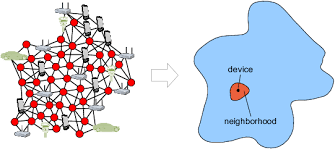
\includegraphics[width=0.5\textwidth]{img/aggregate-computing-structure.png}\\
	{\Huge \textbf{Aggregate Computing}}\\
	{\large Program the \bold{aggregate}, not the individual device} \\[0.2cm]
\end{center}
{\faCircle \, \normalsize{\emph{Computing Machine}} \faArrowRight \, an ensemble of devices as a single body, fading the actual space}\\
{\faCircle \, \normalsize{\emph{Elaboration process}} \faArrowRight \, atomic manipulation of a \emph{collective} data structure (\bold{computational field})}\\
{\faCircle \, \normalsize{\emph{Networked computation}} \faArrowRight \,
a proximity-based self-organising system hidden ``under-the-hood''}
\end{frame}
\begin{frame}{Computational model -- self-organisation-like execution}
\begin{itemize}
	\item \emph{Continuous} communication with \bold{neighbours} only (\faArrowRight decentralisation)
	\item \emph{Continous} execution of async \bold{rounds} of sense - compute - communicate
\end{itemize}
\centering
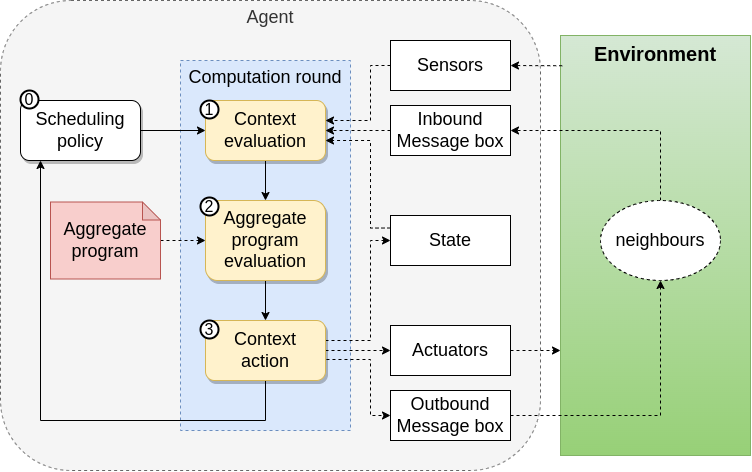
\includegraphics[width=0.8\textwidth]{img/execution-step.png}
\end{frame}

\begin{frame}[fragile]{Applicability: in a nutshell}

Essentially, this approach can be used to program \enf{any} system that can be recast to the following

\begin{itemize}
\item \lbl{Structure:} network of locally interacting agents
	\begin{itemize}
	\item \enf{neighbouring relationship}: e.g. based on network connectivity, physical distance, social relationship, or whatever
	\item \enf{dynamicity/openness}: devices may move/fail, enter/exit the system at runtime, and neighbourhoods may change
	\end{itemize}
\item \lbl{Interaction:} 
	\begin{itemize}
	\item \lbl{with neighbours:} asynchronous message passing
	\item \lbl{with environment:} via sensors and actuators
	\end{itemize}
\item \lbl{Behaviour:} \enf{sense--compute--interact}
	\begin{itemize}
	\item \lbl{sense:} acquire \enf{context} (messages from neigbhours, values from sensors)
	\item \lbl{compute:} mapping context to (inter-)action
	\item \lbl{interact:} sending messages to neighbours and running actuations
	\end{itemize}
\end{itemize}

So, best for applications that are:
\begin{itemize}
\item \enf{progressive/long-running}: require multiple coordinated steps/rounds of local processing and action
\end{itemize}

Assuming this \enf{system model}, AC is about how to specify the ``compute'' part so that \enf{global emergent} outcomes can be eventually attained 

\end{frame}

\begin{frame}[fragile]{Computational Fields: a static view}
	\begin{alertblock}{Traditionally a map: \textit{Space} $\mapsto$ \textit{Values}}
		\begin{itemize}
			\item possibly: evolving over time, dynamically injected, stabilising
			\item smoothly adapting to very heterogeneous domains
			\item more easily \emph{``understood''} on continuous and flat spatial domains
			\item ranging to booleans, reals, vectors, functions
		\end{itemize}
	\end{alertblock}
	\vfill
	\begin{multicols}{3}
		{\fbox{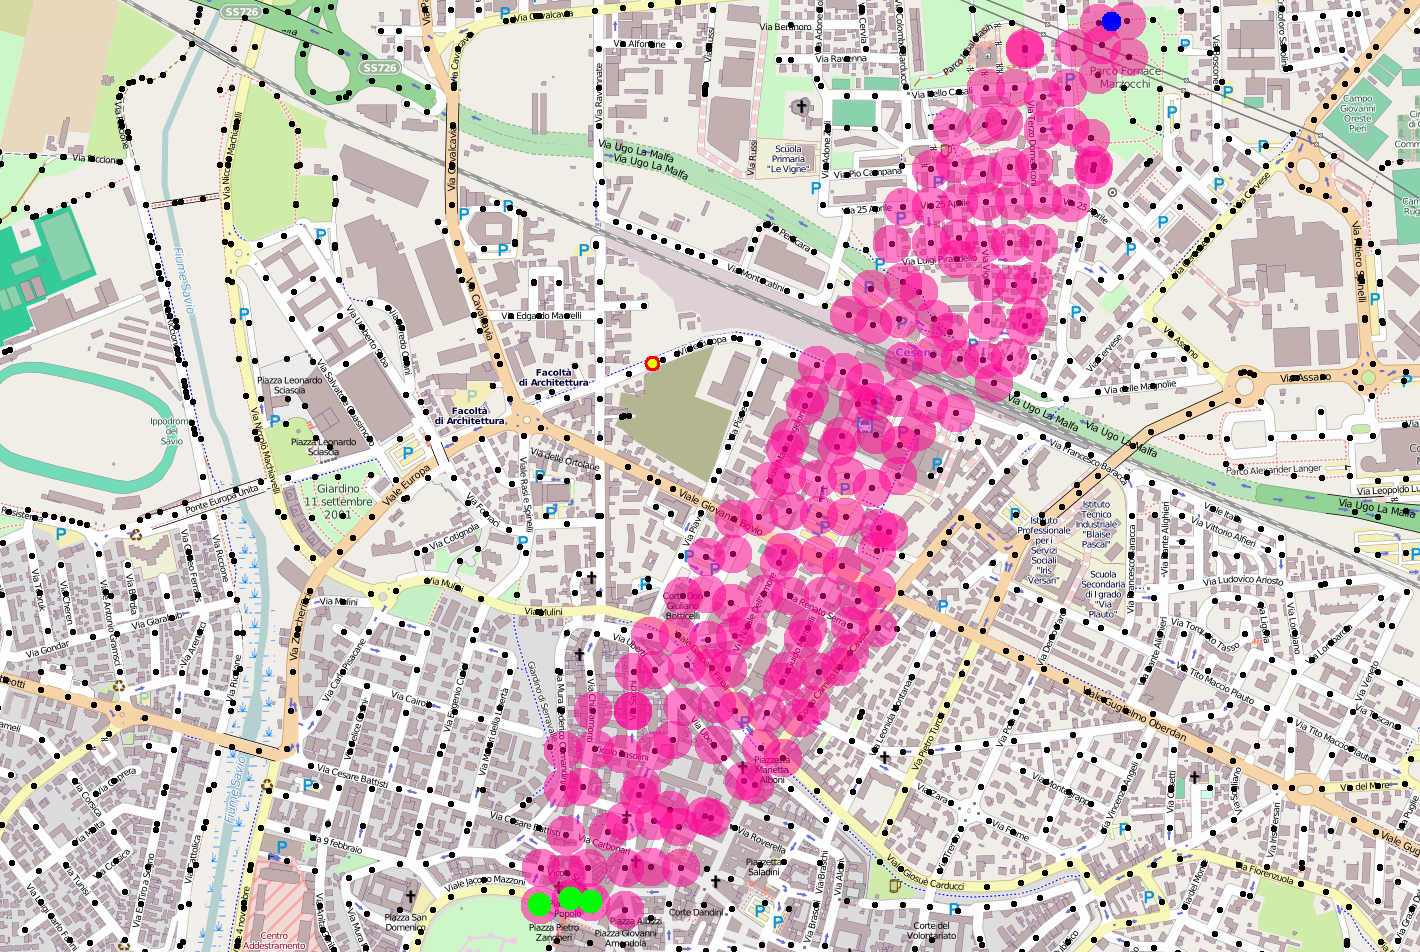
\includegraphics[height=2.3cm]{img/cesena0.png}} boolean channel in 2D}
		{\fbox{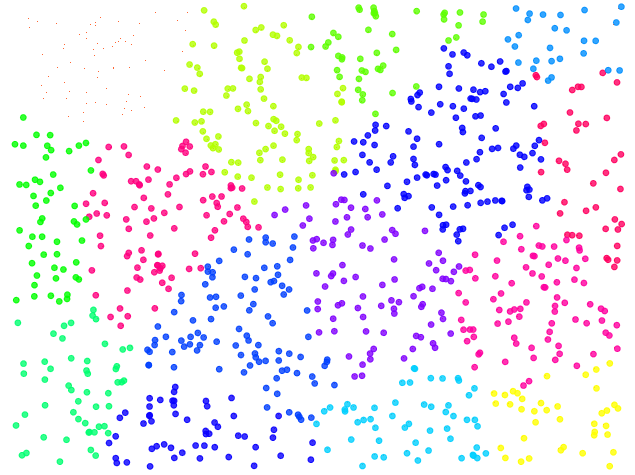
\includegraphics[height=2.3cm]{img/partition.png}} numeric partition in 2D}
		{\fbox{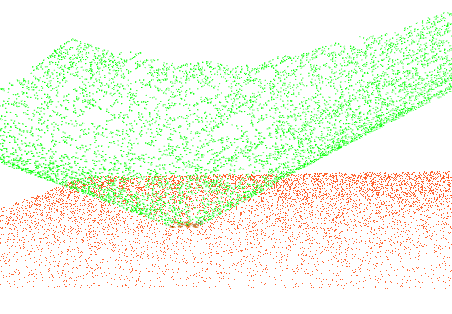
\includegraphics[height=2.3cm]{img/surface2.png}} real-valued gradient in 3D}
	\end{multicols}
\end{frame}
\begin{frame}{Computational Fields revisited: a dynamic view}
\begin{alertblock}{A field as a \textit{space-time} structure: $\phi:D\mapsto V$}
\begin{itemize}
		\item {\it event} $E$: a triple $\langle \delta, t, p\rangle$ -- device $\delta$, ``firing'' at time $t$ in position $p$
		\item {\it events domain} $D$: a coherent set of events (devices cannot move too fast)
		\item {\it field values} $V$: any data value
		\item[\faArrowRight] computation abstracts from/adapts to the underlying event
		\item[\faArrowRight] scheduling of events is essentially exogenous
\end{itemize}
\end{alertblock}
\begin{center}
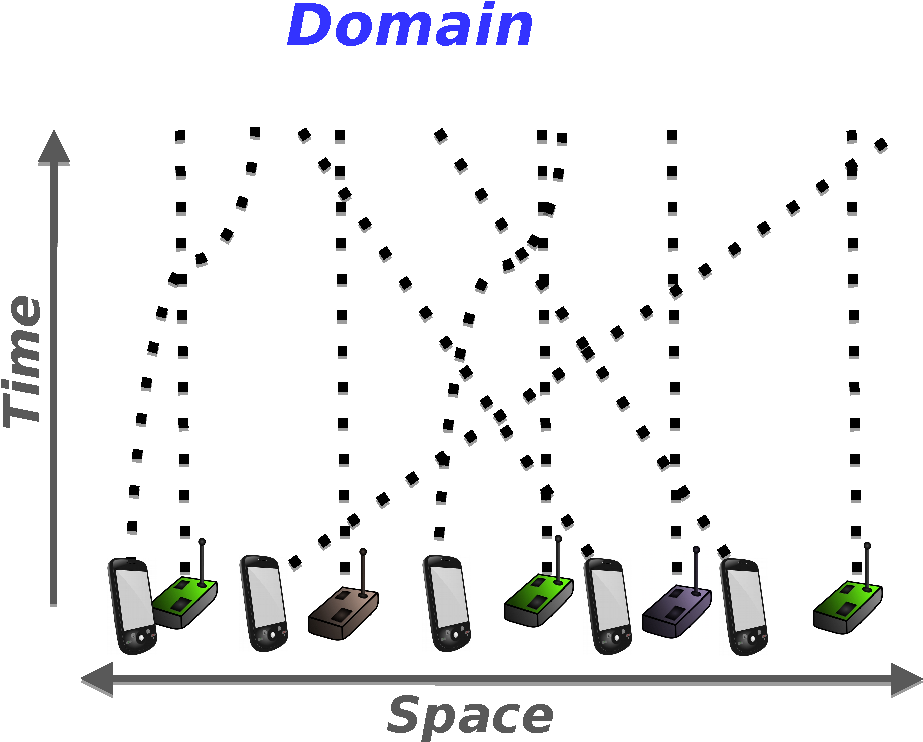
\includegraphics[height=4cm]{img/spacetime1.pdf}~~~~~~~~~~
\only<2->{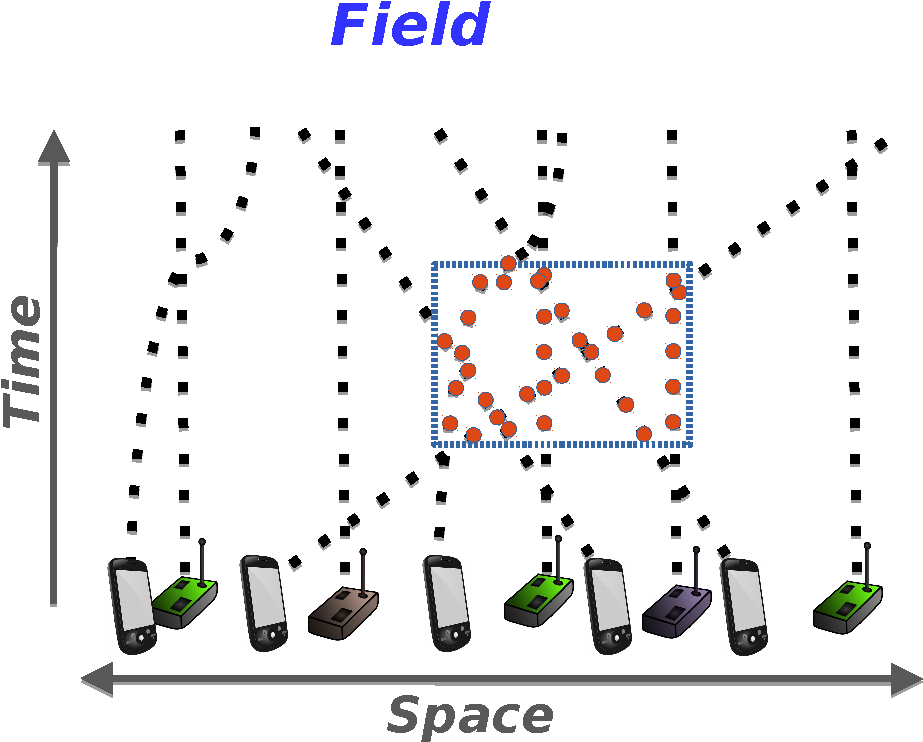
\includegraphics[height=4cm]{img/spacetime2.pdf}} 
\end{center}
\only<3->{will later show only snapshots of fields in 2D space..}
\end{frame}
\begin{frame}{Aggregate programming as a functional approach}
\begin{exampleblock}{Functionally composing fields}
\begin{itemize}
	\item \bold{Inputs}: sensor fields, Output: actuator field
	\item Computation is a pure function over fields (time embeds state!)
	\item[\faArrowRight] for this to be practical/expressive we need a good programming language
\end{itemize}
\end{exampleblock}
\centering
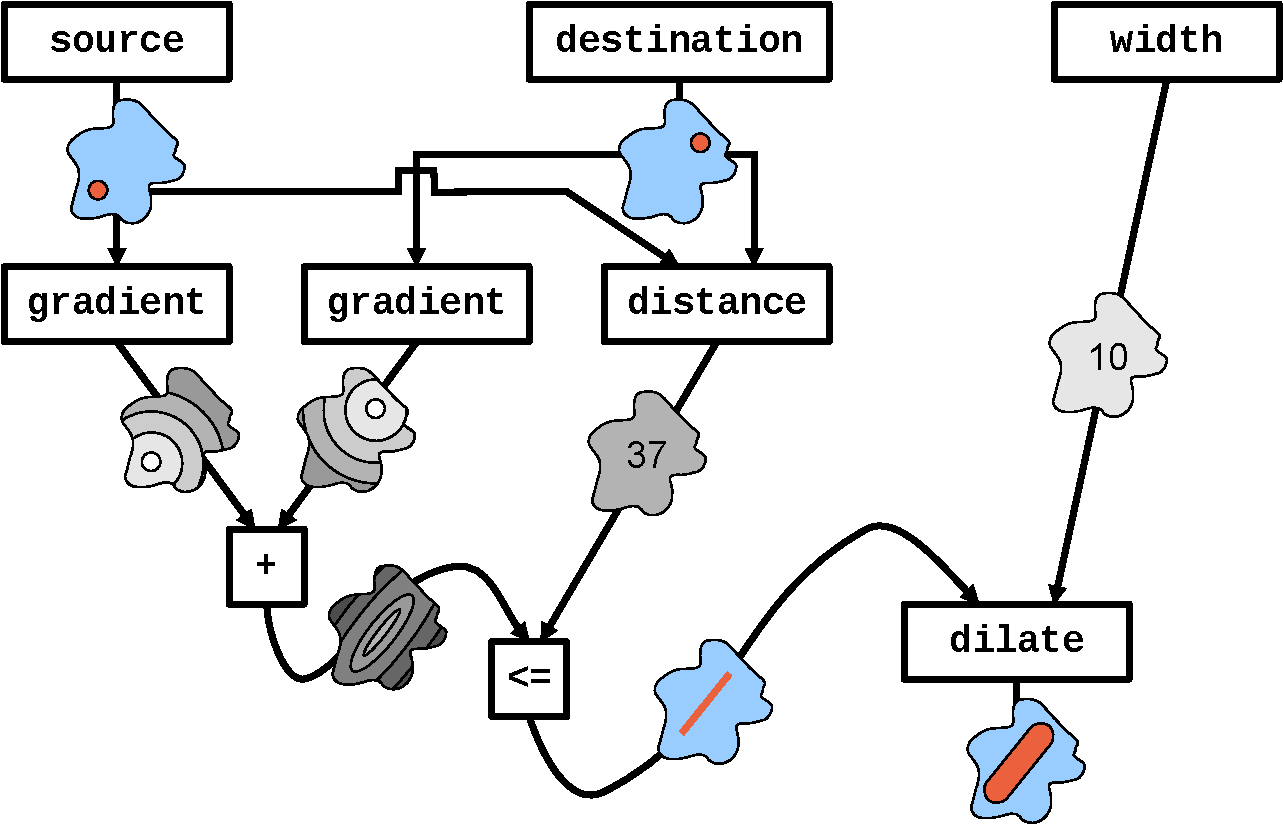
\includegraphics[width=0.65\textwidth]{img/functions.pdf}
\end{frame}
\begin{frame}[fragile]{Preview}
	\begin{exampleblock}{How do we want that computation to be expressed?}
		\begin{itemize}
			\item \texttt{source}, \texttt{dest} and \texttt{width} as inputs
			\item \bold{\texttt{gradient}}, \bold{\texttt{distance}} and \bold{\texttt{dilate}} as reusable functions
			\item[\faArrowRight] note we are reusing and composing global-level, aggregate specs 
		\end{itemize}
	\end{exampleblock}
\centering
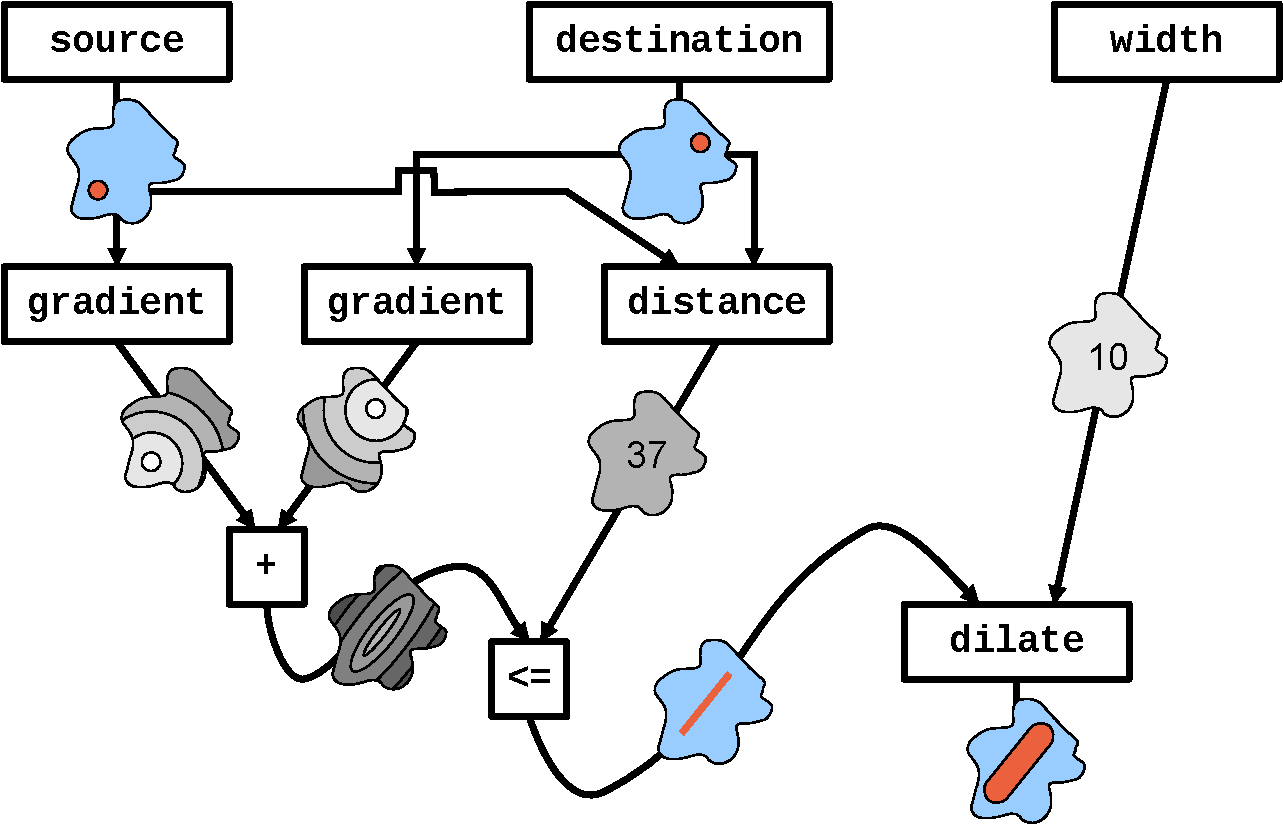
\includegraphics[width=0.45\textwidth]{img/functions.pdf}
\begin{minted}{scala}
def channel(source: Boolean, dest: Boolean, width: Double): Boolean = {
	dilate(gradient(source) + gradient(dest) <= distance(source,dest), width)
}
\end{minted}
\end{frame}
\begin{frame}{Field calculus model}
\begin{exampleblock}{Key idea}
	\begin{itemize}
  \item a sort of $\lambda$-calculus with ``everything is a field'' philosophy!
	\end{itemize}
\end{exampleblock}
\begin{alertblock}{Syntax -- Reduced}
	$\e \;\BNFcce\; \xname 
	\; \BNFmid \; \anyvalue 
%   \;\BNFmid \; \shadow{c\langle\overline\e\rangle}
	\; \BNFmid \; {\e} (\e_1,\ldots,\e_n)
	\;\BNFmid \; \repK(\e_0)\{\e\}
	\; \BNFmid \; \nbrK\{\e\}$\hfill(expr)\\
 $\anyvalue \;\BNFcce \; \textrm{$<$ standard-values $>$} \; \BNFmid \; \lambda $\hfill(value)\\
 $\lambda \;\BNFcce \; \fname \; \BNFmid \; \oname \; \BNFmid \; (\overline{\xname})\texttt{=>}\e$\hfill(functional value)\\
 $\FUNCTION \;\BNFcce \; \defK \; \fname (\overline{\xname}) \; \{\e\}$\hfill(function definition)
\end{alertblock}
\begin{exampleblock}{Few explanations}
	\begin{itemize}
	\item $\anyvalue$ includes numbers, booleans, strings,..\\
	..tuples/vectors/maps/any-ADT (of expressions)
	\item $\fname$ is a user-defined function (the key aggregate computing abstraction)
	\item $\oname$ is a built-in local operator (pure math, local sensors,..)
	\end{itemize}
\end{exampleblock}
\end{frame}

\begin{frame}{Intuition of global-level (denotational) semantics}
	\begin{exampleblock}{The four main constructs at work\\ $\Rightarrow$ values, application, evolution, and interaction -- in aggregate guise}
	\begin{itemize}
		\item $\e \;\BNFcce\; \ldots
   \; \BNFmid \; {\anyvalue}
   \; \BNFmid \; {\e} (\e_1,\ldots,\e_n)
   \;\BNFmid \; \repK(\e_0)\{\e\}
   \; \BNFmid \; \nbrK\{\e\}$
	\end{itemize}
	\end{exampleblock}
\begin{center}
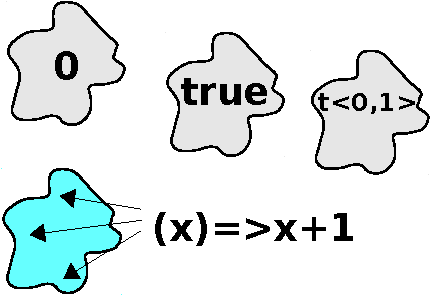
\includegraphics[height=2.3cm]{img/ing-v.pdf}\hspace{30pt}
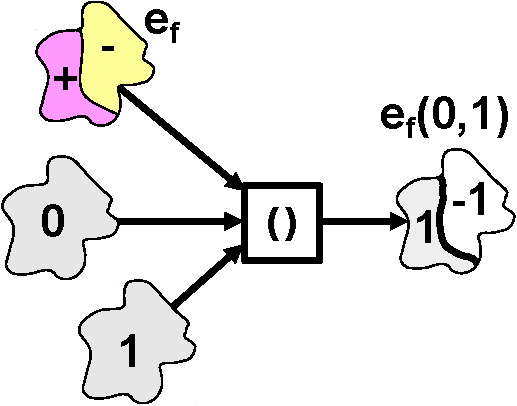
\includegraphics[height=2.57cm]{img/ing-mix5.pdf}\\[5pt]
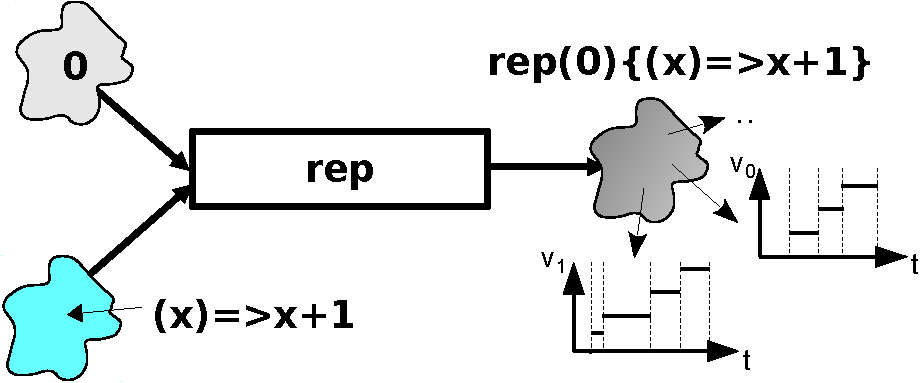
\includegraphics[height=2.42cm]{img/ing-rep2.pdf}\hspace{10pt}
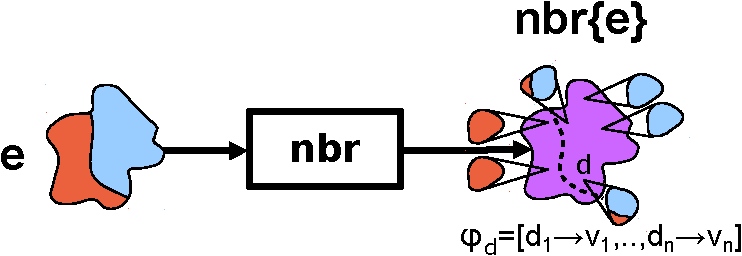
\includegraphics[height=1.96cm]{img/ing-nbr4.pdf}\end{center}
\end{frame}
\begin{frame}[fragile]{Intuition of global-level semantics -- More}
\begin{exampleblock}{Value $\anyvalue$}
	\begin{itemize}
	\item A field constant in space and time, mapping any event to $\anyvalue$
	\end{itemize}
	\end{exampleblock}
	\begin{exampleblock}{Function application ${\e} (\e_1,\ldots,\e_n)$}
	\begin{itemize}
	\item $\e$ evaluates to a field of functions, assume it ranges to $\lambda_1,\ldots,\lambda_n$
	\item this naturally induces a partition of the domain $\domS_1,\ldots,\domS_n$
	\item now, join the fields: $\forall i$, $\lambda_i (\e_1,\ldots,\e_n)$ restricted in $\domS_i$
	\end{itemize}
	\end{exampleblock}
	\begin{exampleblock}{Repetition $\repK(\e_0)\{\e_\lambda\}$}
	\begin{itemize}
	\item the value of $\e_0$ where the restricted domain ``begins''
	\item elsewhere, unary function $\e_\lambda$ is applied to previous value at each device
	\end{itemize}
	\end{exampleblock}
	\begin{exampleblock}{Neighbouring  field construction $\nbrK\{\e\}$}
	\begin{itemize}
	\item at each event gathers most recent value of $\e$ in neighbours (in restriction)
	\item ..what is neighbour is orthogonal (i.e., physical proximity)
	\end{itemize}
	\end{exampleblock}
\end{frame}
\begin{frame}{Key aspects of the semantics: network model}
	\begin{exampleblock}{Platform abstract model}
	\begin{itemize}
			\item A node state $\theta$ (value-tree) updated at asynchronous rounds
			\item At the end of the round, $\theta$ is made accessible to the neighbourhood
			\item A node state is updated ``against'' recently received neighbours' trees
	\end{itemize}
	\end{exampleblock}
	\centering
	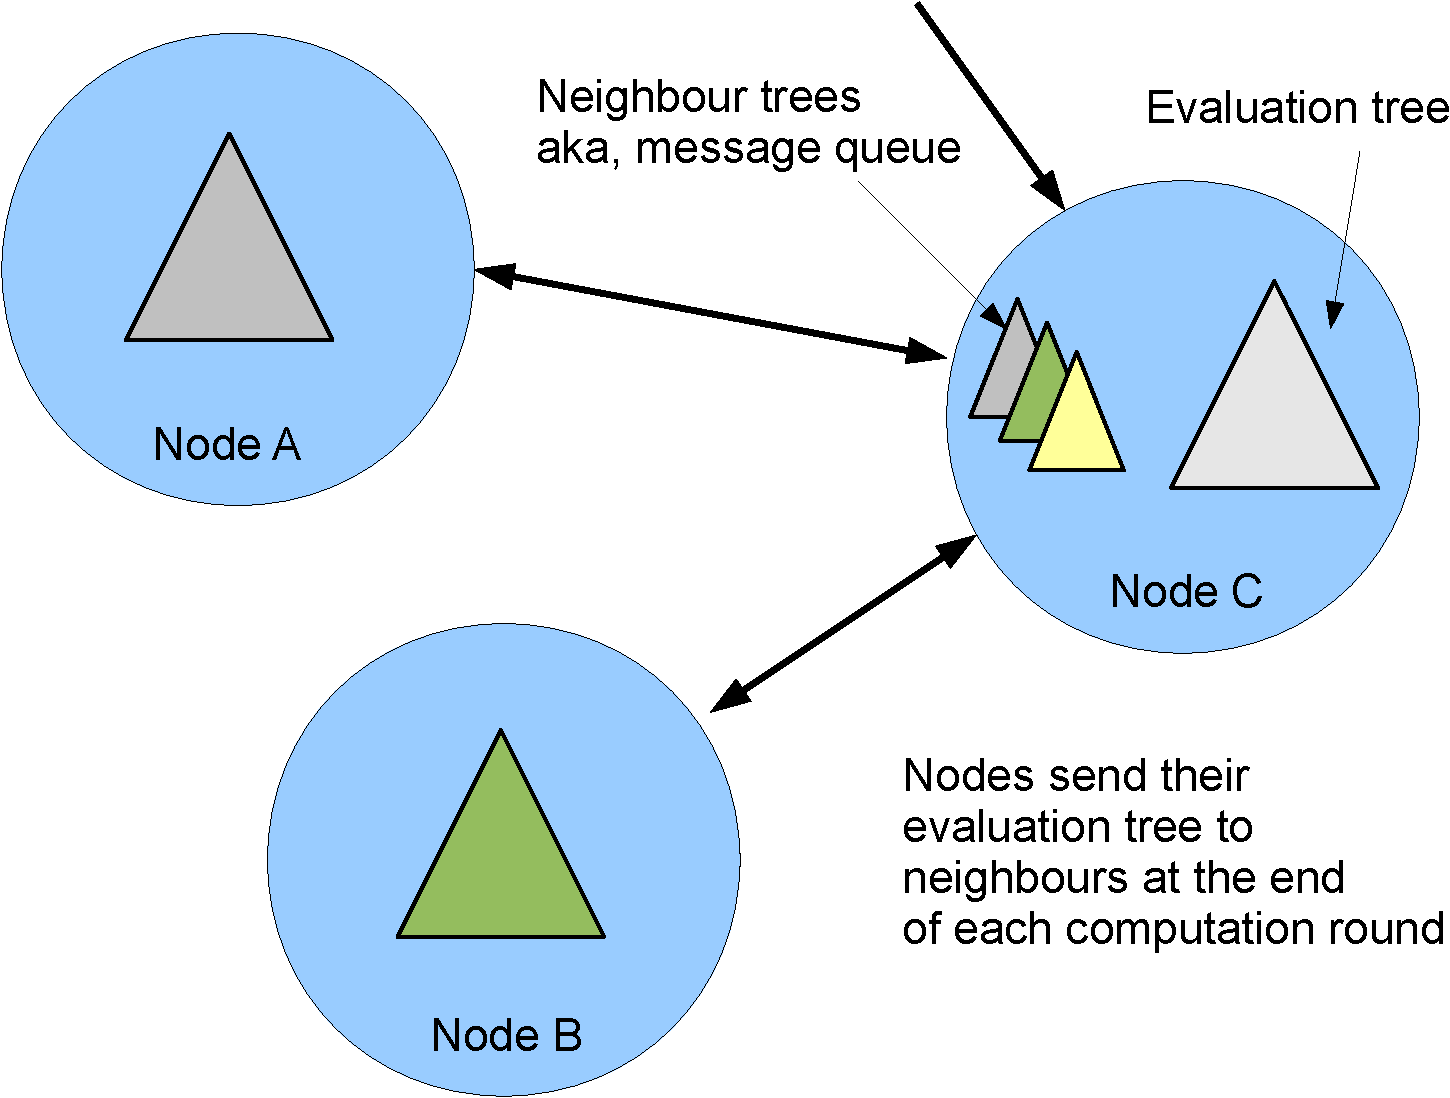
\includegraphics[height=0.5\textheight]{img/nodes.pdf}
	%\fg{height=0.5\textheight}{img/nodes.pdf}
	\end{frame}
	
\begin{frame}[fragile]{Tree evaluation: pictorial semantics}
	\only<1>{
		\centering
		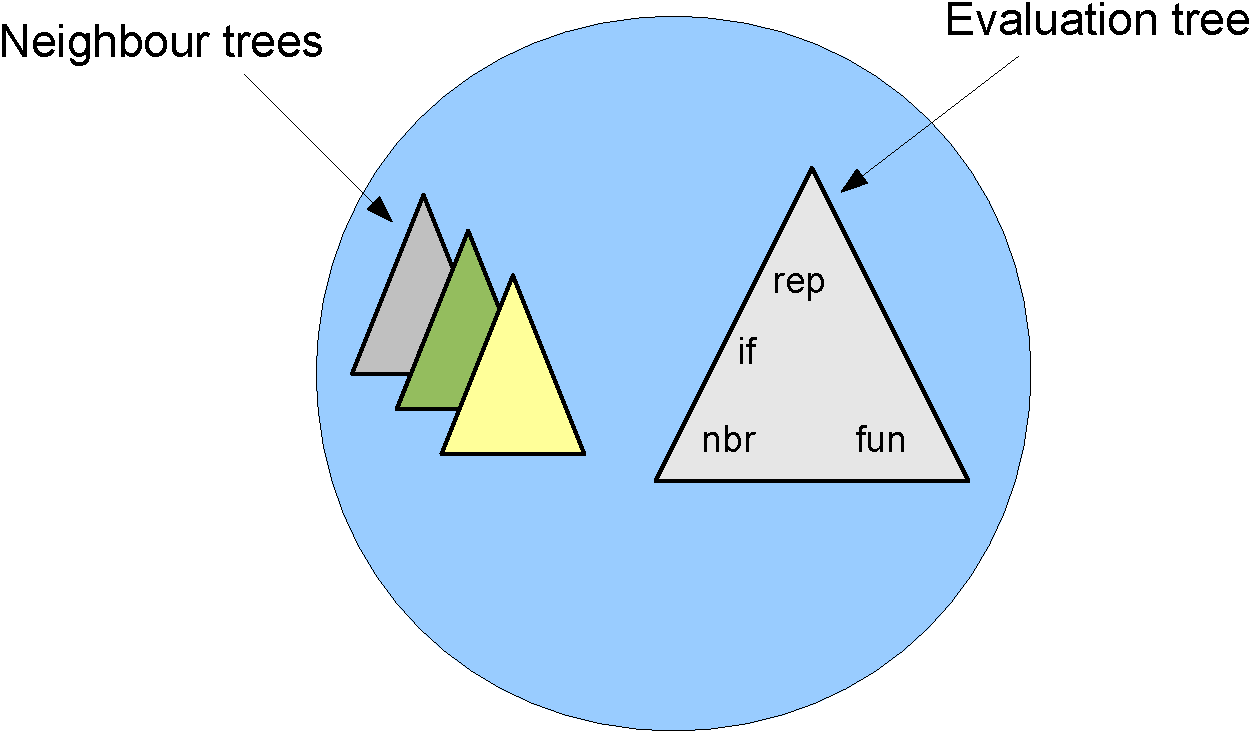
\includegraphics[height=0.75\textheight]{img/tree.pdf}
	}
	\only<2>{
		\centering
		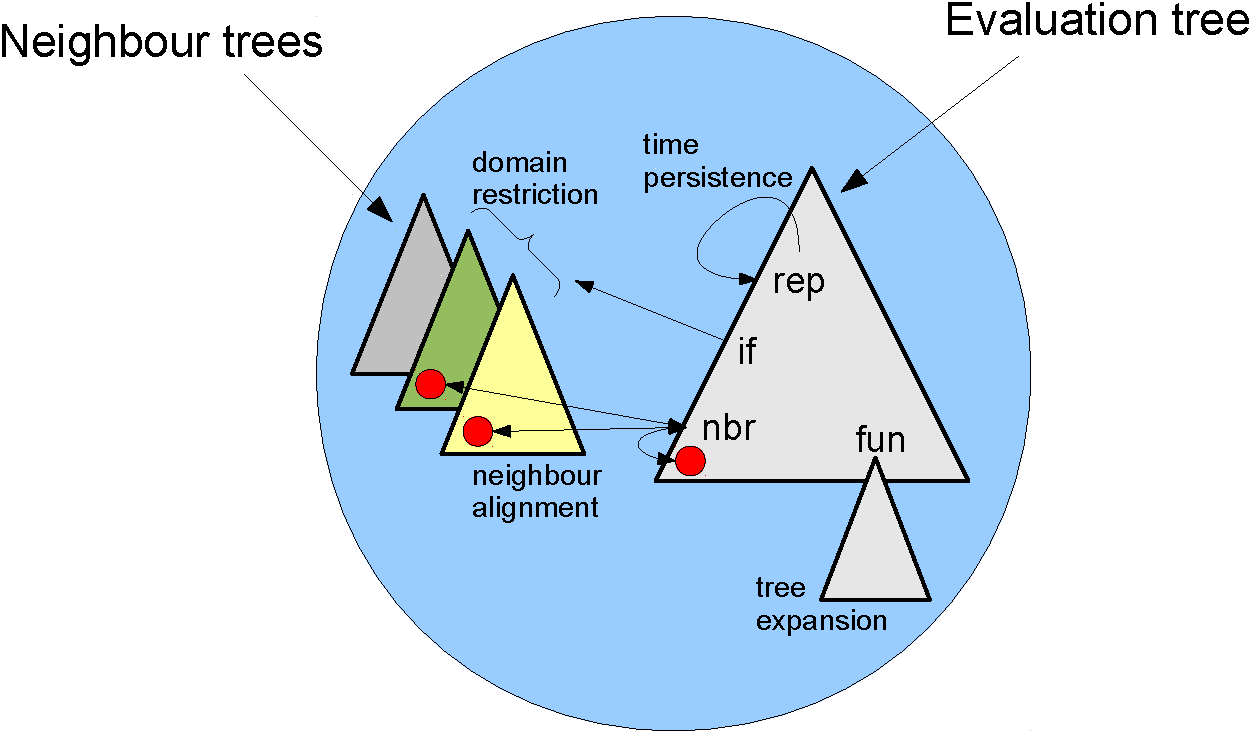
\includegraphics[height=0.75\textheight]{img/tree2.pdf}
	}
	\end{frame}

	\begin{frame}[fragile]{Core mechanisms in the operational semantics}
	\begin{exampleblock}{Orthogonally..}
	\begin{itemize}
	\item evaluation proceeds recursively on expression and neighbour trees
	\item neighbour trees may be discarded on-the-fly if not ``aligned'' (restriction)
	\end{itemize}
	\end{exampleblock}
	\uncover<2->{\begin{exampleblock}{Function application ${\e} (\e_1,\ldots,\e_n)$}
	\begin{itemize}
	\item evaluates the body against a filtered set of neighbours \dots
	\item ..i.e., only those which evaluated $\e$ to the same result
	\end{itemize}
	\end{exampleblock}
	\begin{exampleblock}{Repetition $\repK(\e_0)\{\e_\lambda\}$}
	\begin{itemize}
	\item if a previous value-tree of mine is available, evaluates $\e_\lambda$ on its root
	\item otherwise, evaluates $\e_0$
	\end{itemize}
	\end{exampleblock}
	\begin{exampleblock}{Neighbouring  field construction $\nbrK\{\e\}$}
	\begin{itemize}
	\item gather values from neighbour trees currently aligned
	\item add my current evaluation of $\e$
	\end{itemize}
\end{exampleblock}}
\end{frame}
	
\begin{frame}{Operational semantics as a blueprint for platform support}
	\begin{exampleblock}{Requirements}
	\begin{itemize}
		\item a notion of the neighbourhood must be defined --- wireless connectivity, physical proximity \dots
		\item nodes execute in asynchronous rounds, and emit a ``round result''
		\item a node needs to have recent round results of neighbours
		\item by construction we tolerate losses of messages
		\item by construction we tolerate various round frequencies
	\end{itemize}
	\end{exampleblock}
	\uncover<2->{\begin{exampleblock}{Platform details are very orthogonal to our programming model!}
	\begin{itemize}
		\item the above requirements can be met by various platforms
		\item \emph{programming remains mostly unaltered!}
	\end{itemize}
	\end{exampleblock}}
\end{frame}
	
\begin{frame}[c, plain]
\begin{center}
	
\includegraphics[width=0.2\textwidth]{img/qr-code-scafi.png}\\
	{\Huge \textbf{ScaFi} (\bold{Sca}la \bold{Fi}elds)}\\
	{\large A Scala toolkit providing an \emph{internal domain-specific} language, \emph{libraries}, a \emph{simulation} environment, and \emph{runtime} support for \bold{practical} aggregate computing systems development} \\[0.3cm]
	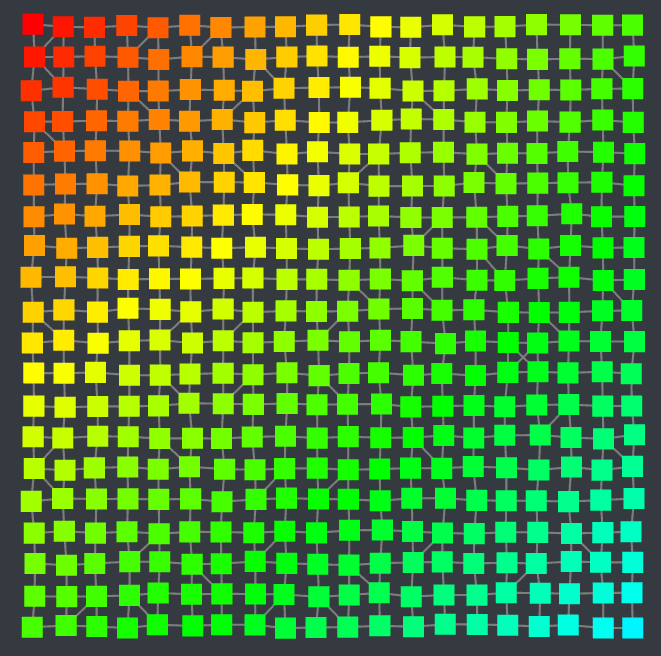
\includegraphics[width=0.2\textwidth]{img/gradient-scafi.png}
	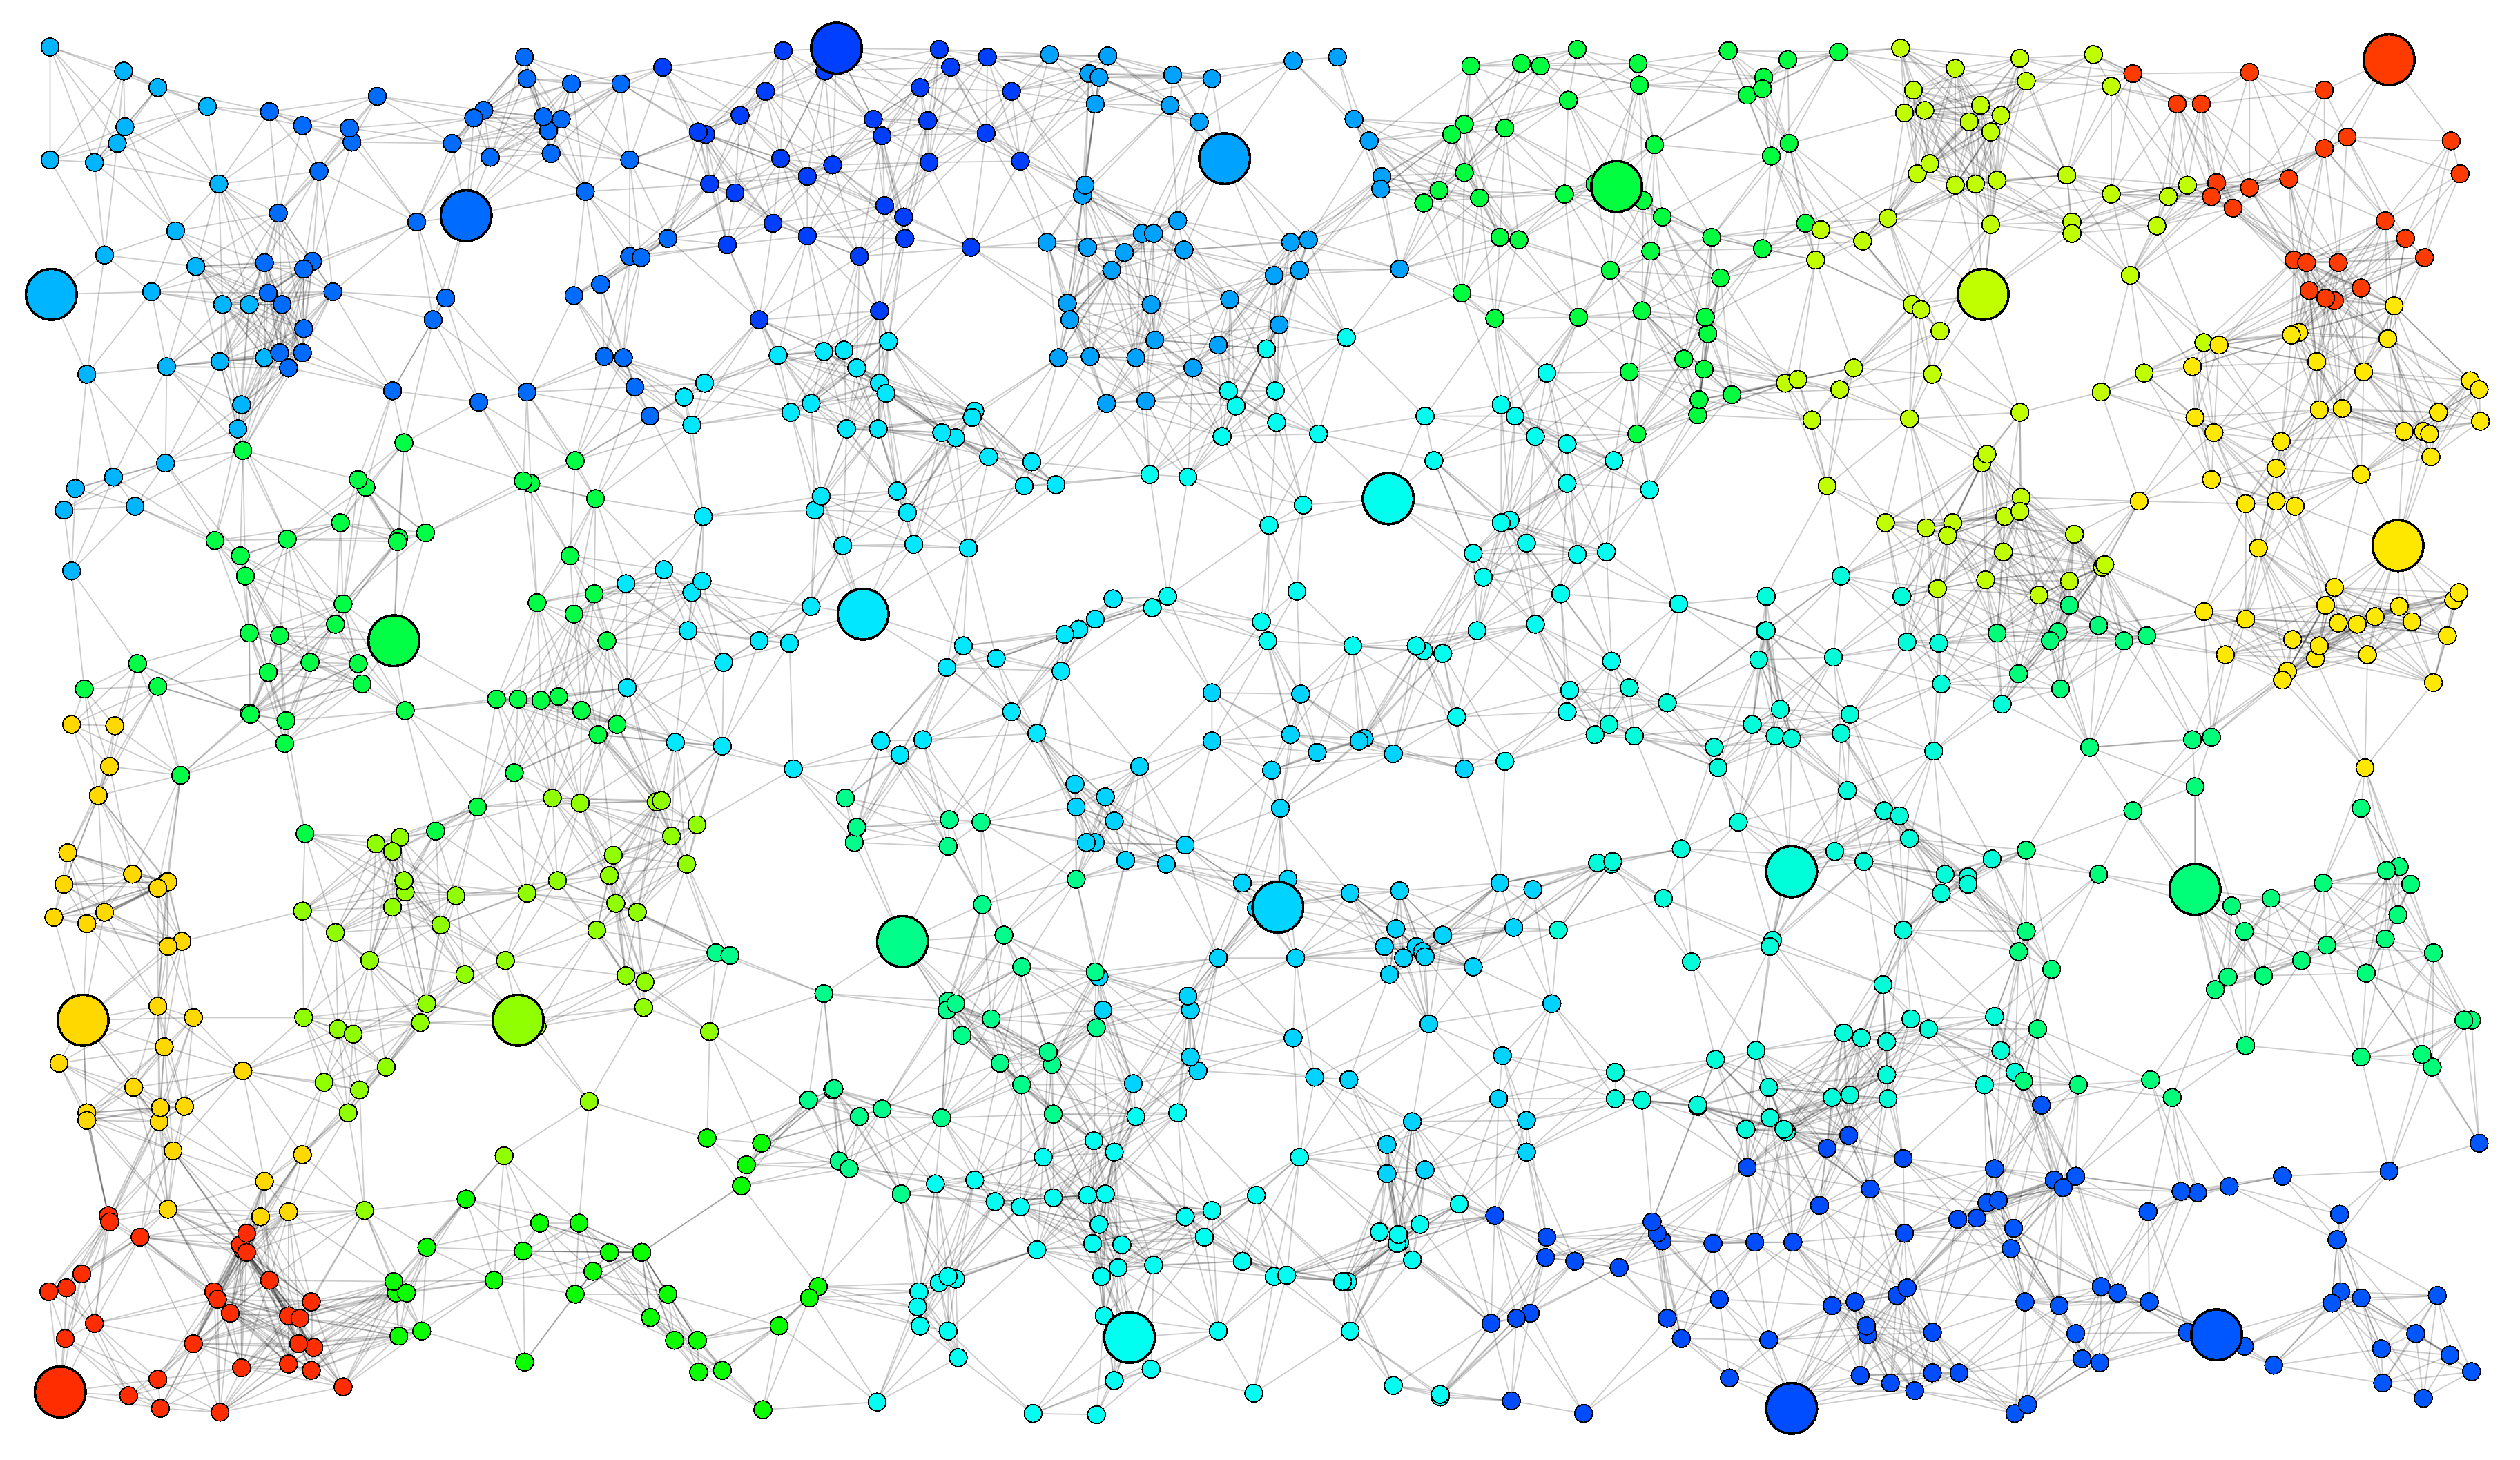
\includegraphics[width=0.35\textwidth]{img/scr-result.png}
	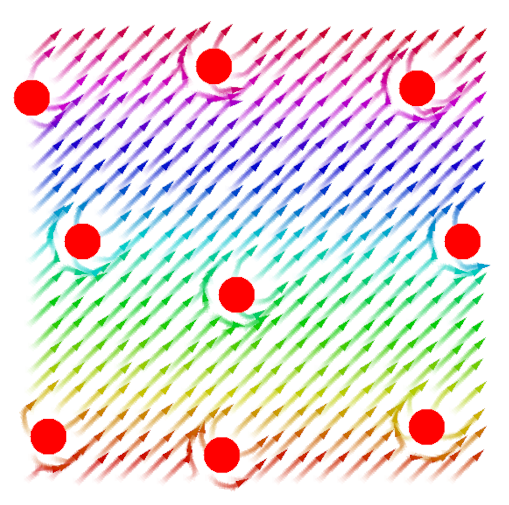
\includegraphics[width=0.215\textwidth]{img/obstacle-avoidance.png}
\end{center}
\end{frame}
\begin{frame}{ScaFi: Organization}
\centering
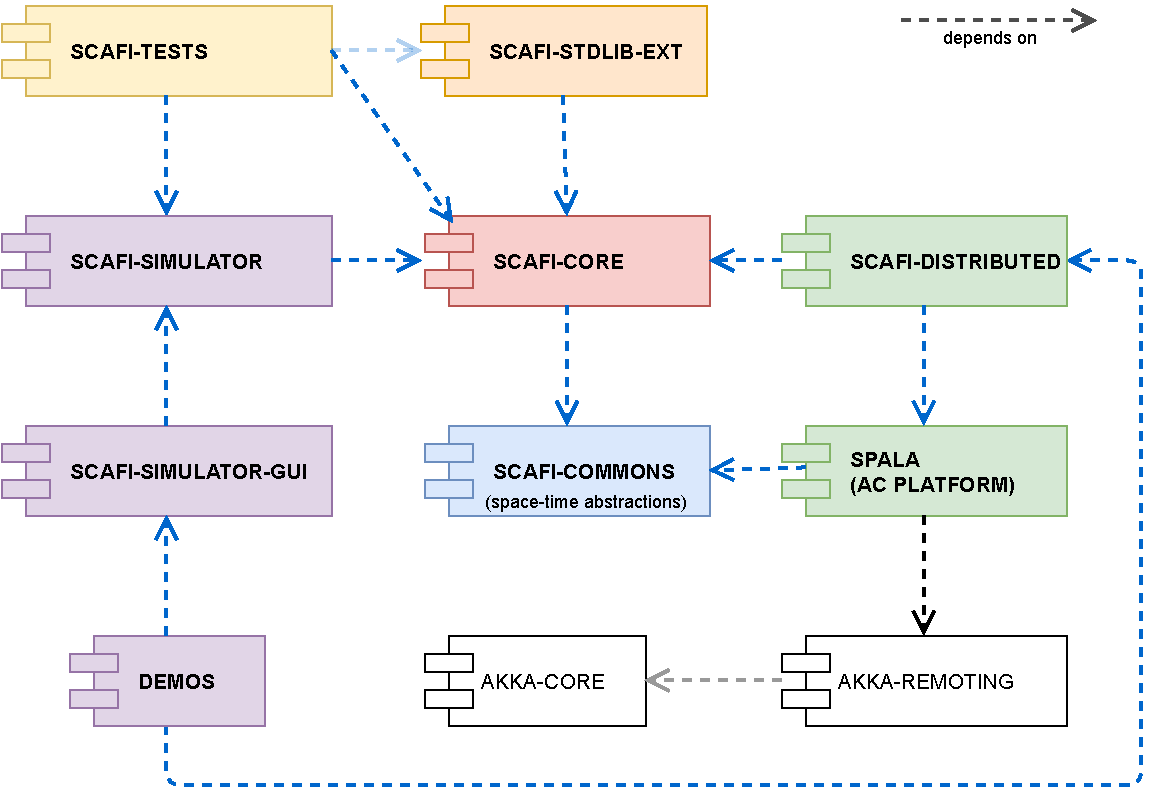
\includegraphics[width=0.9\textwidth]{img/scafi-project-org.pdf}
\end{frame}
\begin{frame}{ScaFi: Design}
\centering
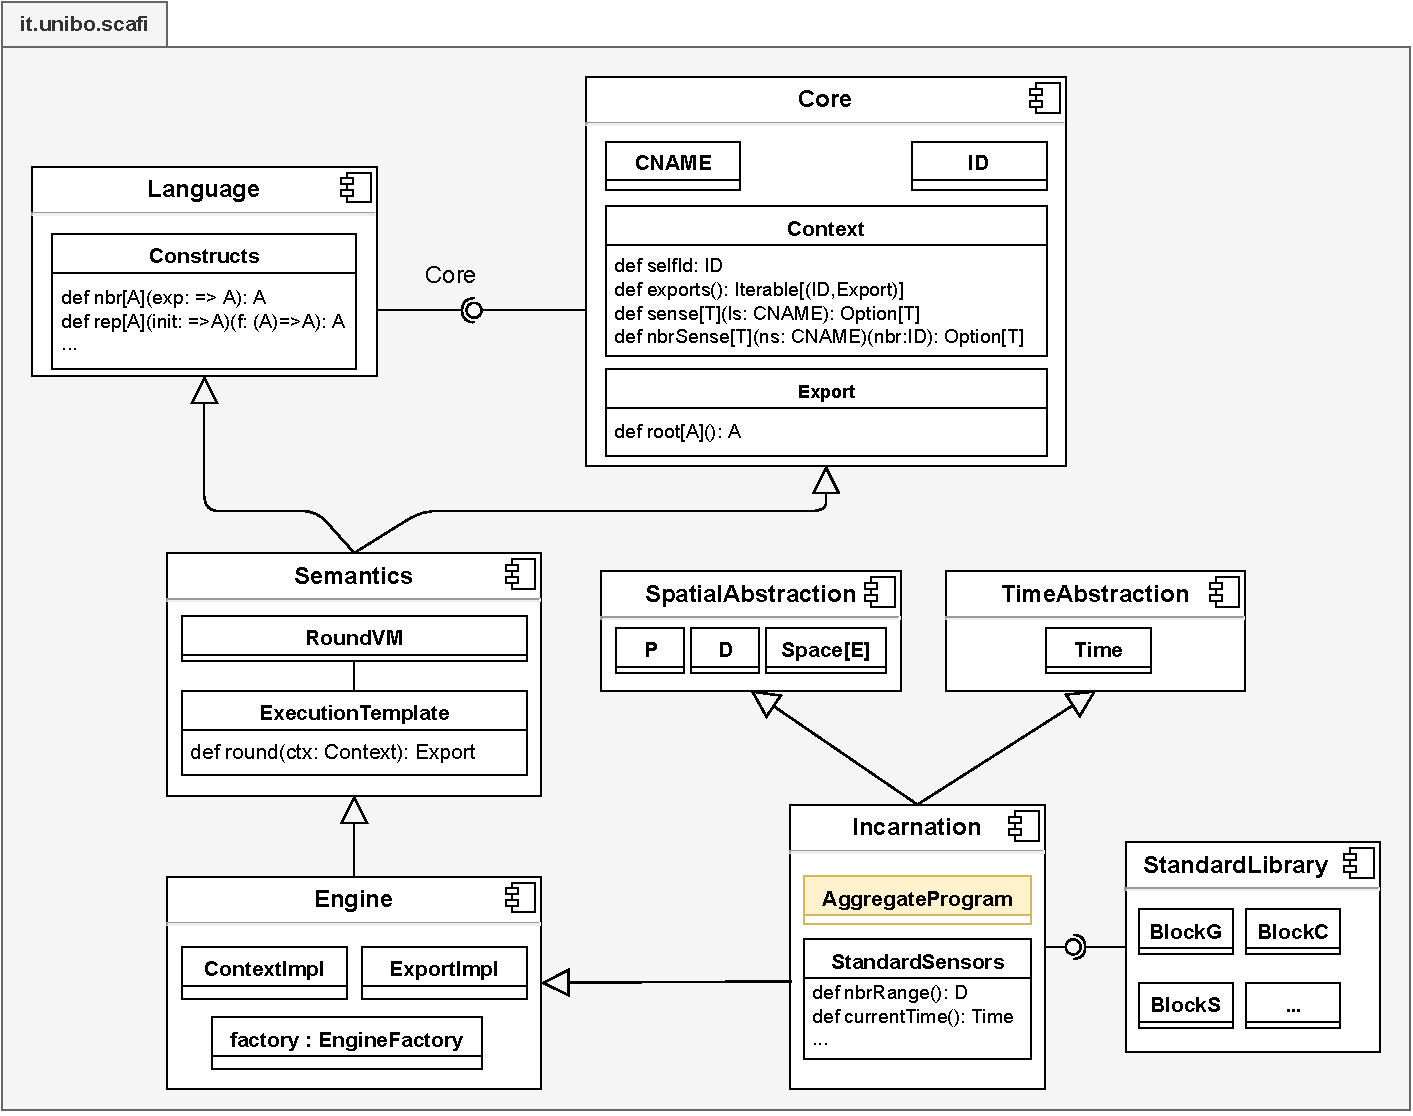
\includegraphics[width=0.8\textwidth]{img/scafi-design.drawio.pdf}
\end{frame}
\begin{frame}[fragile]{ScaFi: syntax as a core language/API}

\begin{minted}{scala}
trait Constructs {
	// the unique identifier of the local device 
	def mid(): ID
	
	// applies fun to the previous result, or to init at the first call
	def rep[A](init: A)(fun: (A) => A): A
	
	// evaluation of expr at the currently-considered neighbour
	def nbr[A](expr: => A): A
	
	// accumulates available evaluations of expr, with acc/init monoid
	def foldhood[A](init: => A)(acc: (A,A)=>A)(expr: => A): A
	
	// splits computation: th where cond is true, el everywhere/time else
	def branch[A](cond: => Boolean)(th: => A)(el: => A): A
	
	// perception of local sensor
	def sense[A](name: CNAME): A
	
	// perception of neighbourhood sensor
	def nbrvar[A](name: CNAME): A
	...
}
\end{minted}
\end{frame}

\begin{frame}[fragile]{ScaFi: setup an aggregate application}

\begin{minted}{scala}
package experiments
// STEP 1 Choose an incarnation (simulated or real)
import it.unibo.scafi.incarnations.BasicSimulationIncarnation._

// STEP 2 Define the aggregate program including the right libraries
class MyProgram extends AggregateProgram with Libs {
	// STEP 2.1 Define main logic of the program
	override def main(): Any = ...
}

// STEP 3 Platform/Node setup (both in simulation/real)

// STEP 3.1 in case of ScaFi simulation:
object SimulationRunner extends Launcher {
  Settings.Sim_ProgramClass = "experiments.MyAggregateProgram"
  Settings.ShowConfigPanel = true
  launch()
}
\end{minted}
\begin{center}
{\huge So let us start playing with ScaFi!! \bold{\faSmileO}}
\end{center}
\end{frame}
%===============================================================================
\section{Playing with ScaFi!}

\begin{frame}{An aggregate computing playground -- ScaFi Web!}
\centering
\url{https://scafi.github.io/web/}
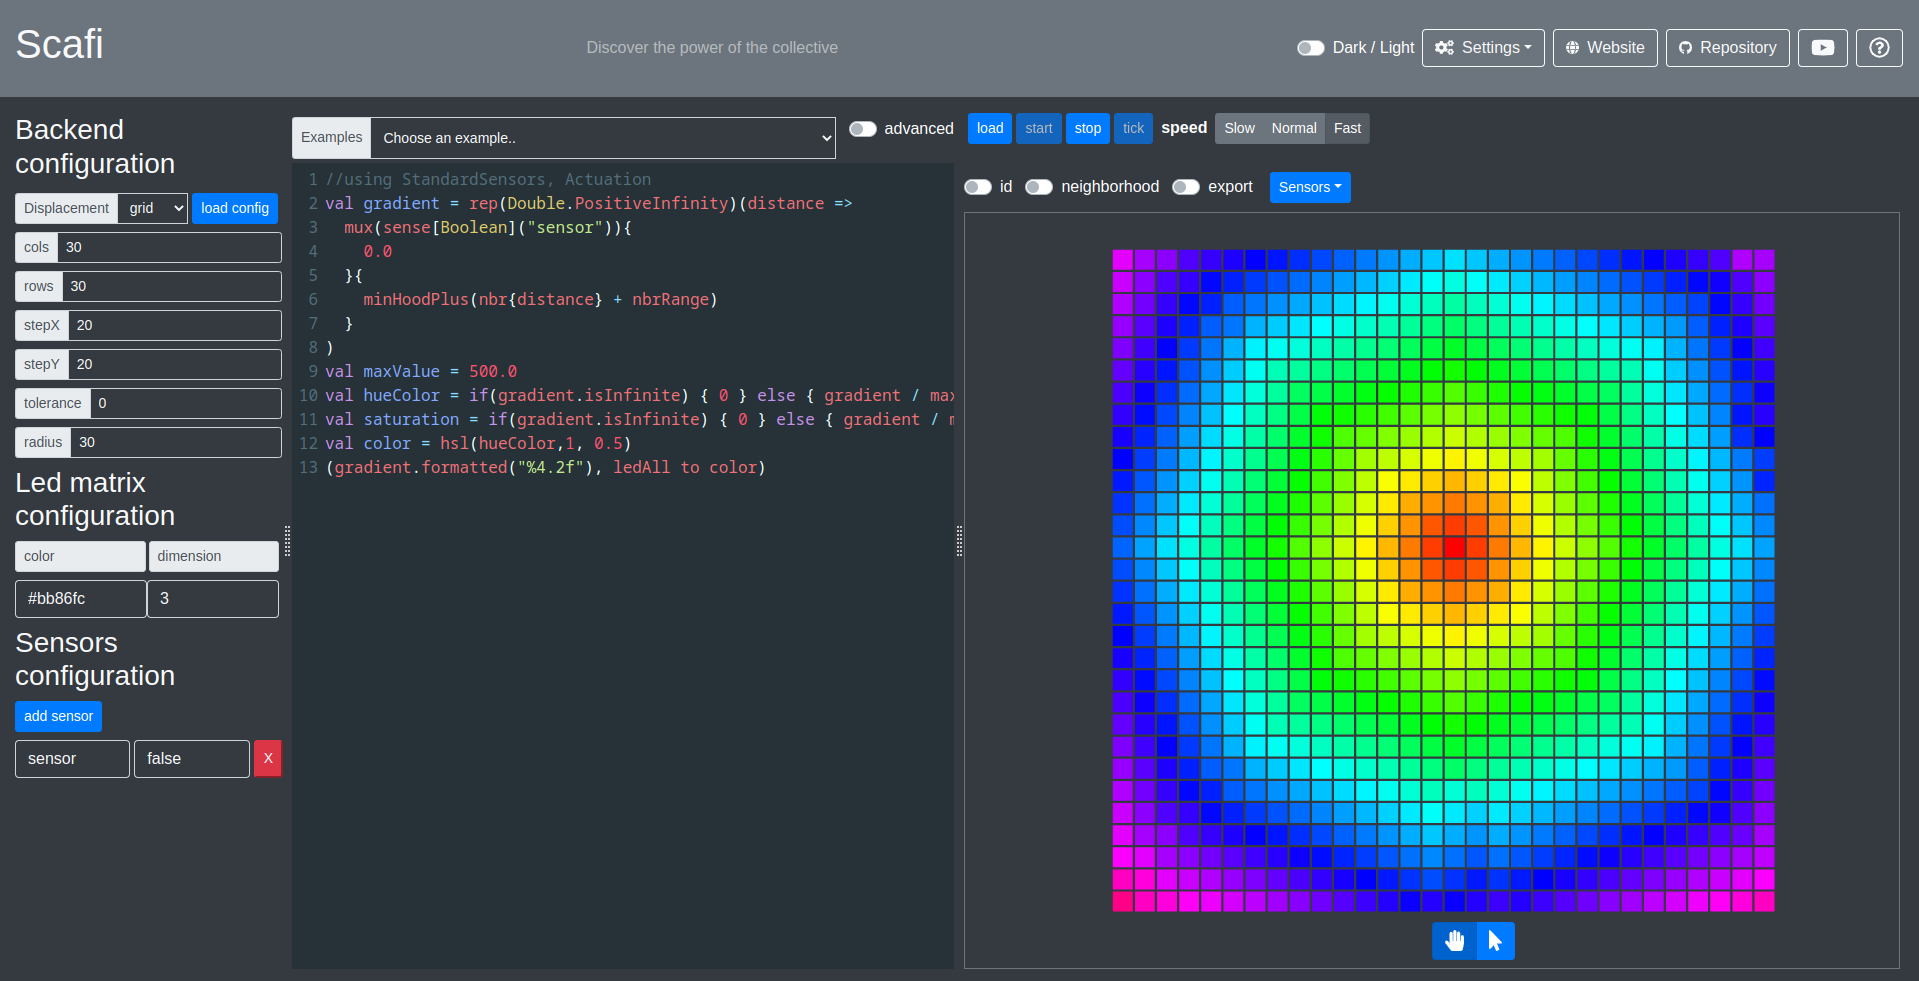
\includegraphics[width=\textwidth]{img/gradient-web.png}
\end{frame}
\section{ScaFi in real-world scenarios: Integration with Alchemist}
\subsection{Alchemist}
\begin{frame}[c, plain]
\begin{center}
	
\includegraphics[width=0.2\textwidth]{img/qr-code.png}\\
	\Huge \textbf{Alchemist}\\
	{\large An \bold{extensible} \emph{meta}-simulator for \textbf{pervasive} computing scenarios}\\[0.3cm]
	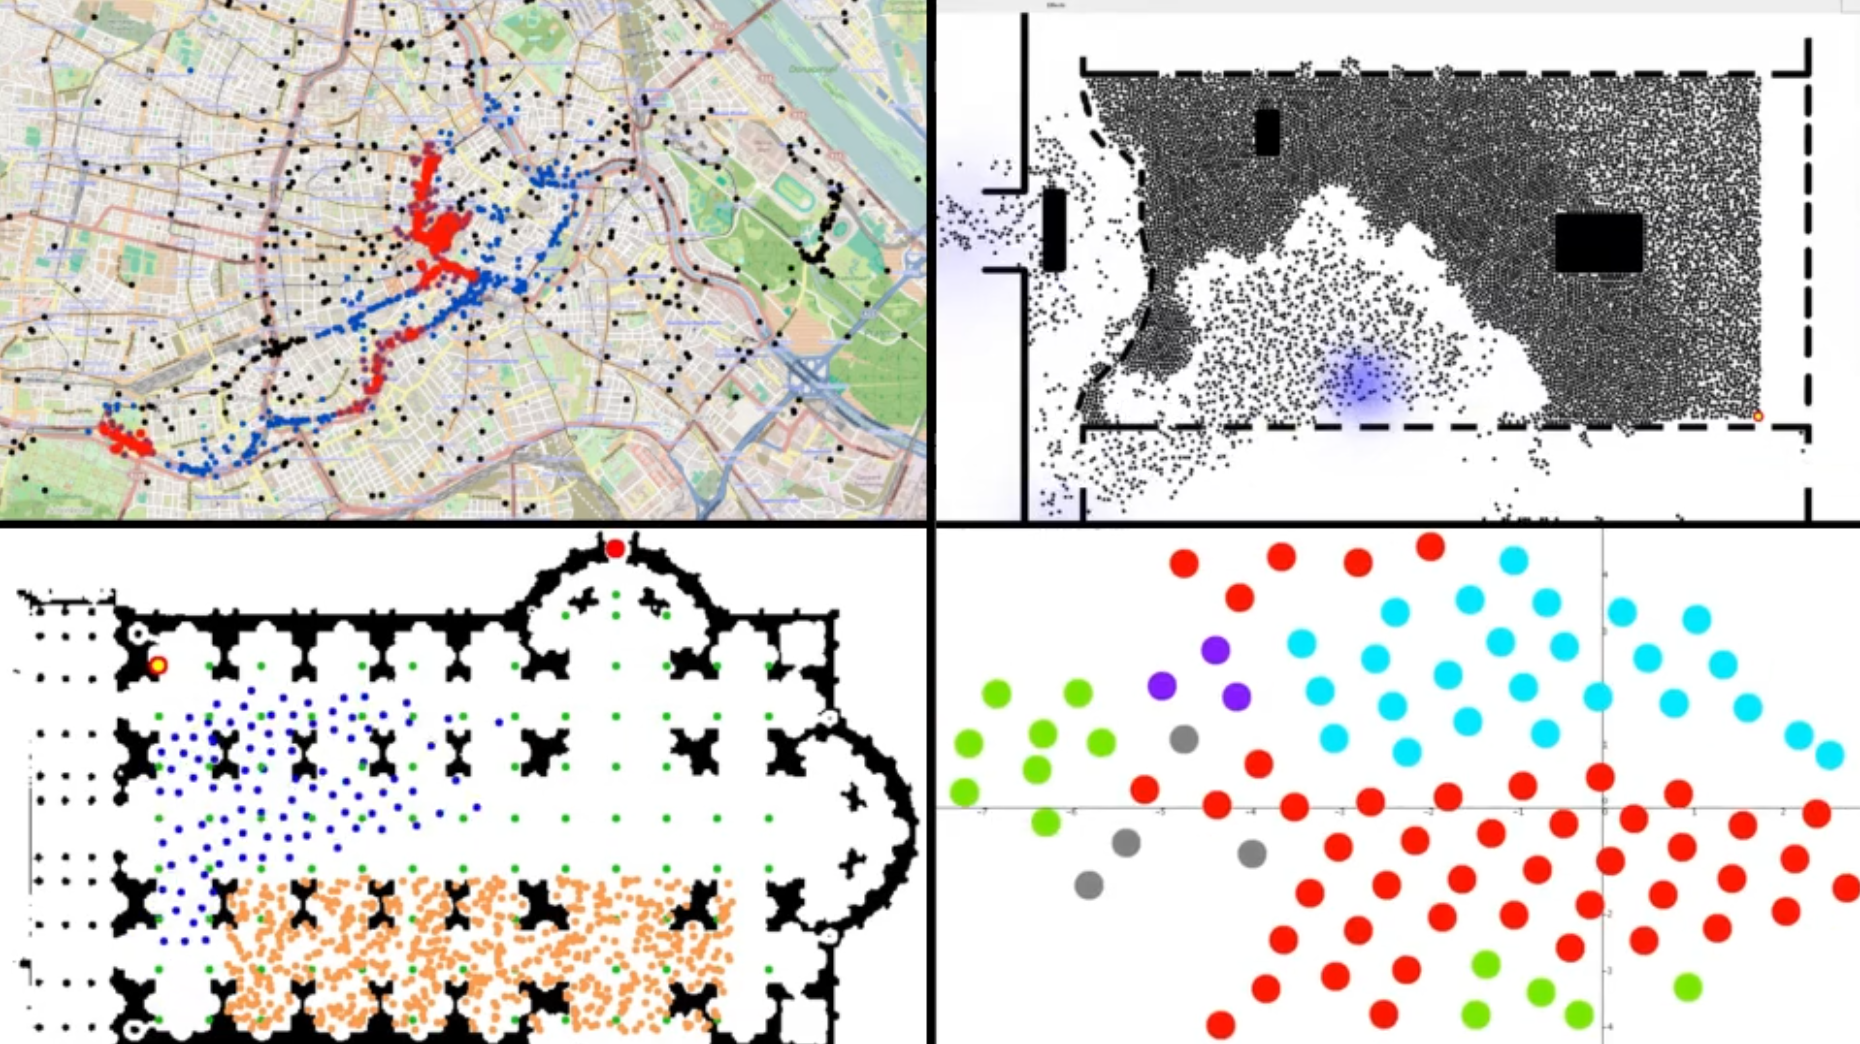
\includegraphics[width=0.5\textwidth]{img/alchemist-recap.png}
\end{center}
\end{frame}
\begin{frame}{Abstract model}
\centering
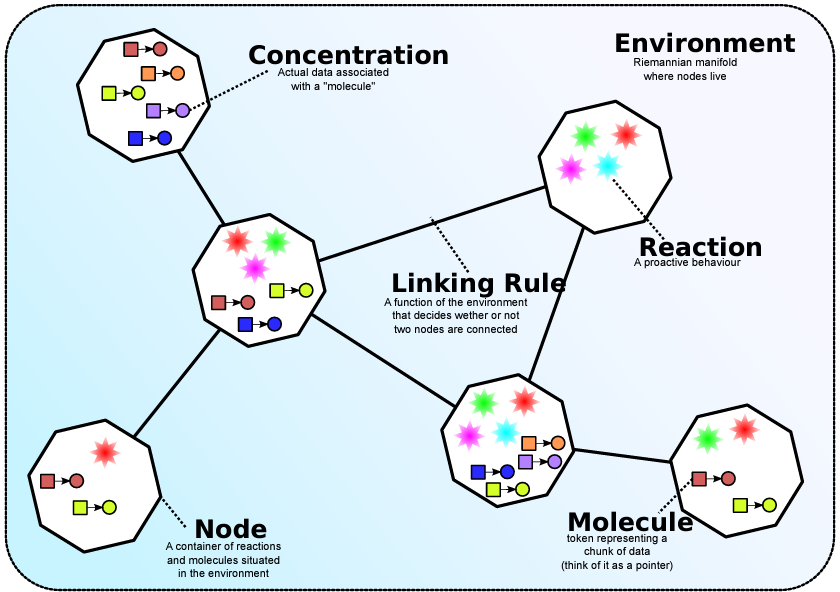
\includegraphics[width=0.8\textwidth]{img/abstract-model.png}
\end{frame}
\begin{frame}{Reactions}
\centering
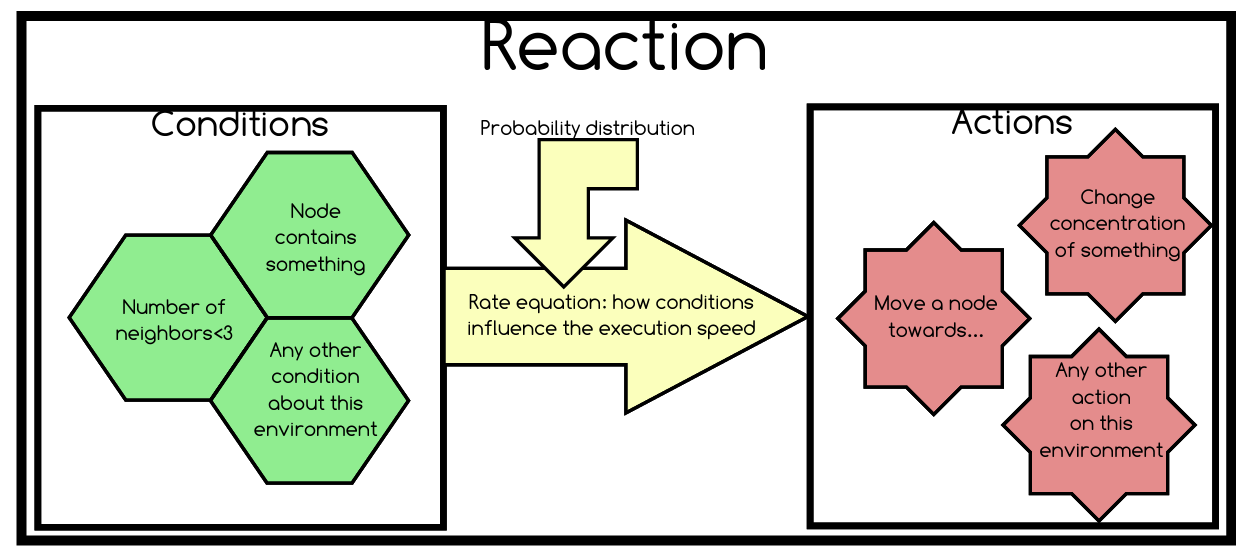
\includegraphics[width=0.8\textwidth]{img/reaction-model.png}
\end{frame}
\begin{frame}{Overall Architecture}
\centering
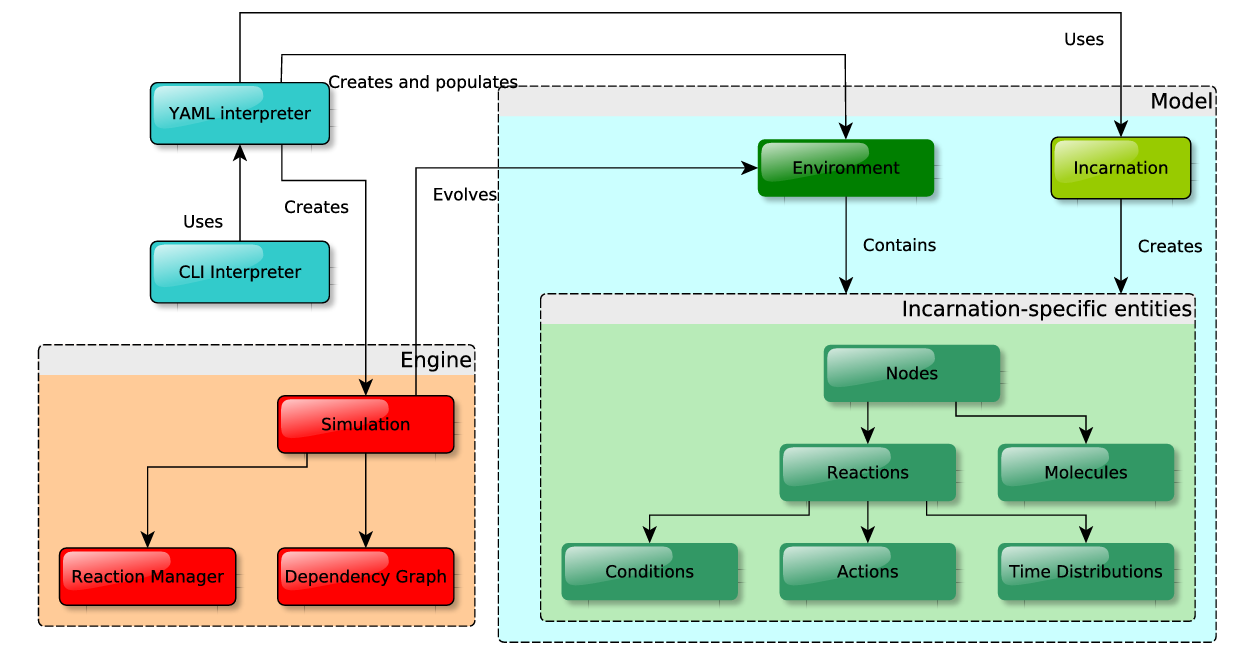
\includegraphics[width=0.8\textwidth]{img/alchemist-architecture.png}
\end{frame}
\begin{frame}{ScaFi Incarnation}
\begin{block}{Motivation}
	\begin{itemize}
		\item ScaFi has its own simulator \dots
		\item \dots but it is not as powerful as Alchemist, which:
		\begin{itemize}
			\item support GPS traces
			\item can simulate thousands of nodes
			\item can simulate different kinds of networks
			\item can simulate different mobility models
		\end{itemize}
	\end{itemize}
\end{block}
\begin{exampleblock}{ScaFi-Alchemist known uses}
	\begin{itemize}
		\item Swarm Robotics API: MacroSwarm\footnote[frame]{\fullcite{macroswarm}}
		\item Large-Scale smart cities simulations: FloodWatch\footnote[frame]{\fullcite{iee-floodwatch}}
		\item Crowd simulations
		\item \dots
	\end{itemize}
\end{exampleblock}
\end{frame}
\begin{frame}{Writing Simulations with ScaFi incarnation}
\begin{itemize}
	\item Alchemist uses YAML\footnote{\url{https://learnxinyminutes.com/docs/yaml/}} as language for writing simulations
	\begin{itemize}
		\item YAML is a human-readable data-serialization language
		\item It is a superset of JSON
		\item Support anchors and references
	\end{itemize}
	\item The same syntax is used for \bold{any} incarnations
	\item Support running in \bold{batch}
	\item No compilation is needed 
	\begin{itemize}
		\item[\faThumbsUp] Once you have your ScaFi script compiled, you can run it in several alchemist simulations!!
	\end{itemize}
	\item Support ad-hoc export of simulation data through CSV files. 
\end{itemize}
\end{frame}
\begin{frame}[fragile]{Minimal specification}
\begin{minted}{yaml}
incarnation: scafi
\end{minted}
\end{frame}
\begin{frame}[fragile]{Node displacement and connection}
\begin{minted}{yaml}
incarnation: scafi
network-model:
  type: ConnectWithinDistance
  parameters: [0.5]

# More deployments at 
# https://alchemistsimulator.github.io/howtos/simulation/deploy
deployments: # Description of where the nodes should be
  type: Grid
  parameters: [-5, -5, 5, 5, 0.25, 0.25, 0, 0]
\end{minted}
\end{frame}
\begin{frame}[fragile]{Node Content}
	\begin{minted}{yaml}
incarnation: scafi
network-model:
  type: ConnectWithinDistance
  parameters: [0.5]

deployments: # Description of where the nodes should be
  type: Grid
  parameters: [-5, -5, 5, 5, 0.25, 0.25, 0, 0]
  contents:
	  - molecule: data
		  value: 0
	  - in:
		  	type: Rectangle
		  	parameters: [-1, -1, 2, 2]
		  molecule: source
\end{minted}
\end{frame}
\section{Aggregate Computing -- Research Profiles}
\begin{frame}{Swarm Robotics}

\end{frame}

\begin{frame}{\st{Multi} Many agent reinforcement}
\end{frame}
\section{}

%===============================================================================

%/////////
\frame{\titlepage}
%/////////

%===============================================================================
\section*{\refname}
%===============================================================================

%%%%
\setbeamertemplate{page number in head/foot}{}
%/////////


\begin{frame}[allowframebreaks]{References}
\def\bibfont{\footnotesize}
\printbibliography
\end{frame}

%%%%%%%%%%%%%%%%%%%%%%%%%%%%%%%%%%%%%%%%%%%%%%%%%%%%%%%%%%%%%%%%%%%%%%%%%%%%%%%%
\end{document}
%%%%%%%%%%%%%%%%%%%%%%%%%%%%%%%%%%%%%%%%%%%%%%%%%%%%%%%%%%%%%%%%%%%%%%%%%%%%%%%%
